% Options for packages loaded elsewhere
\PassOptionsToPackage{unicode}{hyperref}
\PassOptionsToPackage{hyphens}{url}
\PassOptionsToPackage{dvipsnames,svgnames,x11names}{xcolor}
%
\documentclass[
  letterpaper,
  DIV=11,
  numbers=noendperiod]{scrreprt}

\usepackage{amsmath,amssymb}
\usepackage{iftex}
\ifPDFTeX
  \usepackage[T1]{fontenc}
  \usepackage[utf8]{inputenc}
  \usepackage{textcomp} % provide euro and other symbols
\else % if luatex or xetex
  \usepackage{unicode-math}
  \defaultfontfeatures{Scale=MatchLowercase}
  \defaultfontfeatures[\rmfamily]{Ligatures=TeX,Scale=1}
\fi
\usepackage{lmodern}
\ifPDFTeX\else  
    % xetex/luatex font selection
\fi
% Use upquote if available, for straight quotes in verbatim environments
\IfFileExists{upquote.sty}{\usepackage{upquote}}{}
\IfFileExists{microtype.sty}{% use microtype if available
  \usepackage[]{microtype}
  \UseMicrotypeSet[protrusion]{basicmath} % disable protrusion for tt fonts
}{}
\makeatletter
\@ifundefined{KOMAClassName}{% if non-KOMA class
  \IfFileExists{parskip.sty}{%
    \usepackage{parskip}
  }{% else
    \setlength{\parindent}{0pt}
    \setlength{\parskip}{6pt plus 2pt minus 1pt}}
}{% if KOMA class
  \KOMAoptions{parskip=half}}
\makeatother
\usepackage{xcolor}
\setlength{\emergencystretch}{3em} % prevent overfull lines
\setcounter{secnumdepth}{5}
% Make \paragraph and \subparagraph free-standing
\ifx\paragraph\undefined\else
  \let\oldparagraph\paragraph
  \renewcommand{\paragraph}[1]{\oldparagraph{#1}\mbox{}}
\fi
\ifx\subparagraph\undefined\else
  \let\oldsubparagraph\subparagraph
  \renewcommand{\subparagraph}[1]{\oldsubparagraph{#1}\mbox{}}
\fi

\usepackage{color}
\usepackage{fancyvrb}
\newcommand{\VerbBar}{|}
\newcommand{\VERB}{\Verb[commandchars=\\\{\}]}
\DefineVerbatimEnvironment{Highlighting}{Verbatim}{commandchars=\\\{\}}
% Add ',fontsize=\small' for more characters per line
\usepackage{framed}
\definecolor{shadecolor}{RGB}{241,243,245}
\newenvironment{Shaded}{\begin{snugshade}}{\end{snugshade}}
\newcommand{\AlertTok}[1]{\textcolor[rgb]{0.68,0.00,0.00}{#1}}
\newcommand{\AnnotationTok}[1]{\textcolor[rgb]{0.37,0.37,0.37}{#1}}
\newcommand{\AttributeTok}[1]{\textcolor[rgb]{0.40,0.45,0.13}{#1}}
\newcommand{\BaseNTok}[1]{\textcolor[rgb]{0.68,0.00,0.00}{#1}}
\newcommand{\BuiltInTok}[1]{\textcolor[rgb]{0.00,0.23,0.31}{#1}}
\newcommand{\CharTok}[1]{\textcolor[rgb]{0.13,0.47,0.30}{#1}}
\newcommand{\CommentTok}[1]{\textcolor[rgb]{0.37,0.37,0.37}{#1}}
\newcommand{\CommentVarTok}[1]{\textcolor[rgb]{0.37,0.37,0.37}{\textit{#1}}}
\newcommand{\ConstantTok}[1]{\textcolor[rgb]{0.56,0.35,0.01}{#1}}
\newcommand{\ControlFlowTok}[1]{\textcolor[rgb]{0.00,0.23,0.31}{#1}}
\newcommand{\DataTypeTok}[1]{\textcolor[rgb]{0.68,0.00,0.00}{#1}}
\newcommand{\DecValTok}[1]{\textcolor[rgb]{0.68,0.00,0.00}{#1}}
\newcommand{\DocumentationTok}[1]{\textcolor[rgb]{0.37,0.37,0.37}{\textit{#1}}}
\newcommand{\ErrorTok}[1]{\textcolor[rgb]{0.68,0.00,0.00}{#1}}
\newcommand{\ExtensionTok}[1]{\textcolor[rgb]{0.00,0.23,0.31}{#1}}
\newcommand{\FloatTok}[1]{\textcolor[rgb]{0.68,0.00,0.00}{#1}}
\newcommand{\FunctionTok}[1]{\textcolor[rgb]{0.28,0.35,0.67}{#1}}
\newcommand{\ImportTok}[1]{\textcolor[rgb]{0.00,0.46,0.62}{#1}}
\newcommand{\InformationTok}[1]{\textcolor[rgb]{0.37,0.37,0.37}{#1}}
\newcommand{\KeywordTok}[1]{\textcolor[rgb]{0.00,0.23,0.31}{#1}}
\newcommand{\NormalTok}[1]{\textcolor[rgb]{0.00,0.23,0.31}{#1}}
\newcommand{\OperatorTok}[1]{\textcolor[rgb]{0.37,0.37,0.37}{#1}}
\newcommand{\OtherTok}[1]{\textcolor[rgb]{0.00,0.23,0.31}{#1}}
\newcommand{\PreprocessorTok}[1]{\textcolor[rgb]{0.68,0.00,0.00}{#1}}
\newcommand{\RegionMarkerTok}[1]{\textcolor[rgb]{0.00,0.23,0.31}{#1}}
\newcommand{\SpecialCharTok}[1]{\textcolor[rgb]{0.37,0.37,0.37}{#1}}
\newcommand{\SpecialStringTok}[1]{\textcolor[rgb]{0.13,0.47,0.30}{#1}}
\newcommand{\StringTok}[1]{\textcolor[rgb]{0.13,0.47,0.30}{#1}}
\newcommand{\VariableTok}[1]{\textcolor[rgb]{0.07,0.07,0.07}{#1}}
\newcommand{\VerbatimStringTok}[1]{\textcolor[rgb]{0.13,0.47,0.30}{#1}}
\newcommand{\WarningTok}[1]{\textcolor[rgb]{0.37,0.37,0.37}{\textit{#1}}}

\providecommand{\tightlist}{%
  \setlength{\itemsep}{0pt}\setlength{\parskip}{0pt}}\usepackage{longtable,booktabs,array}
\usepackage{calc} % for calculating minipage widths
% Correct order of tables after \paragraph or \subparagraph
\usepackage{etoolbox}
\makeatletter
\patchcmd\longtable{\par}{\if@noskipsec\mbox{}\fi\par}{}{}
\makeatother
% Allow footnotes in longtable head/foot
\IfFileExists{footnotehyper.sty}{\usepackage{footnotehyper}}{\usepackage{footnote}}
\makesavenoteenv{longtable}
\usepackage{graphicx}
\makeatletter
\def\maxwidth{\ifdim\Gin@nat@width>\linewidth\linewidth\else\Gin@nat@width\fi}
\def\maxheight{\ifdim\Gin@nat@height>\textheight\textheight\else\Gin@nat@height\fi}
\makeatother
% Scale images if necessary, so that they will not overflow the page
% margins by default, and it is still possible to overwrite the defaults
% using explicit options in \includegraphics[width, height, ...]{}
\setkeys{Gin}{width=\maxwidth,height=\maxheight,keepaspectratio}
% Set default figure placement to htbp
\makeatletter
\def\fps@figure{htbp}
\makeatother
% definitions for citeproc citations
\NewDocumentCommand\citeproctext{}{}
\NewDocumentCommand\citeproc{mm}{%
  \begingroup\def\citeproctext{#2}\cite{#1}\endgroup}
\makeatletter
 % allow citations to break across lines
 \let\@cite@ofmt\@firstofone
 % avoid brackets around text for \cite:
 \def\@biblabel#1{}
 \def\@cite#1#2{{#1\if@tempswa , #2\fi}}
\makeatother
\newlength{\cslhangindent}
\setlength{\cslhangindent}{1.5em}
\newlength{\csllabelwidth}
\setlength{\csllabelwidth}{3em}
\newenvironment{CSLReferences}[2] % #1 hanging-indent, #2 entry-spacing
 {\begin{list}{}{%
  \setlength{\itemindent}{0pt}
  \setlength{\leftmargin}{0pt}
  \setlength{\parsep}{0pt}
  % turn on hanging indent if param 1 is 1
  \ifodd #1
   \setlength{\leftmargin}{\cslhangindent}
   \setlength{\itemindent}{-1\cslhangindent}
  \fi
  % set entry spacing
  \setlength{\itemsep}{#2\baselineskip}}}
 {\end{list}}
\usepackage{calc}
\newcommand{\CSLBlock}[1]{\hfill\break\parbox[t]{\linewidth}{\strut\ignorespaces#1\strut}}
\newcommand{\CSLLeftMargin}[1]{\parbox[t]{\csllabelwidth}{\strut#1\strut}}
\newcommand{\CSLRightInline}[1]{\parbox[t]{\linewidth - \csllabelwidth}{\strut#1\strut}}
\newcommand{\CSLIndent}[1]{\hspace{\cslhangindent}#1}

\KOMAoption{captions}{tableheading}
\makeatletter
\@ifpackageloaded{bookmark}{}{\usepackage{bookmark}}
\makeatother
\makeatletter
\@ifpackageloaded{caption}{}{\usepackage{caption}}
\AtBeginDocument{%
\ifdefined\contentsname
  \renewcommand*\contentsname{Table of contents}
\else
  \newcommand\contentsname{Table of contents}
\fi
\ifdefined\listfigurename
  \renewcommand*\listfigurename{List of Figures}
\else
  \newcommand\listfigurename{List of Figures}
\fi
\ifdefined\listtablename
  \renewcommand*\listtablename{List of Tables}
\else
  \newcommand\listtablename{List of Tables}
\fi
\ifdefined\figurename
  \renewcommand*\figurename{Figure}
\else
  \newcommand\figurename{Figure}
\fi
\ifdefined\tablename
  \renewcommand*\tablename{Table}
\else
  \newcommand\tablename{Table}
\fi
}
\@ifpackageloaded{float}{}{\usepackage{float}}
\floatstyle{ruled}
\@ifundefined{c@chapter}{\newfloat{codelisting}{h}{lop}}{\newfloat{codelisting}{h}{lop}[chapter]}
\floatname{codelisting}{Listing}
\newcommand*\listoflistings{\listof{codelisting}{List of Listings}}
\makeatother
\makeatletter
\makeatother
\makeatletter
\@ifpackageloaded{caption}{}{\usepackage{caption}}
\@ifpackageloaded{subcaption}{}{\usepackage{subcaption}}
\makeatother
\ifLuaTeX
  \usepackage{selnolig}  % disable illegal ligatures
\fi
\usepackage{bookmark}

\IfFileExists{xurl.sty}{\usepackage{xurl}}{} % add URL line breaks if available
\urlstyle{same} % disable monospaced font for URLs
\hypersetup{
  pdftitle={Proof of concept for health indicators},
  pdfauthor={Julian Flowers},
  colorlinks=true,
  linkcolor={blue},
  filecolor={Maroon},
  citecolor={Blue},
  urlcolor={Blue},
  pdfcreator={LaTeX via pandoc}}

\title{Proof of concept for health indicators}
\author{Julian Flowers}
\date{2024-07-12}

\begin{document}
\maketitle

\renewcommand*\contentsname{Table of contents}
{
\hypersetup{linkcolor=}
\setcounter{tocdepth}{2}
\tableofcontents
}
\bookmarksetup{startatroot}

\chapter{Introduction}\label{introduction}

Outline an end-to-end process for creating public health indicators and
generating public health profiles.

\begin{figure}

\centering{

\includegraphics[width=6.43in,height=6.65in]{index_files/figure-latex/mermaid-figure-1.png}

}

\caption{\label{fig-comp}Workflow}

\end{figure}%

\bookmarksetup{startatroot}

\chapter{Rapid EDA}\label{rapid-eda}

A first step is to rapidly evaluate raw data.

In creating regional health indicators and profiles

Store data in a single directory

\begin{Shaded}
\begin{Highlighting}[]
\NormalTok{dir }\OtherTok{\textless{}{-}} \FunctionTok{here}\NormalTok{(}\StringTok{"data"}\NormalTok{)}

\NormalTok{xl\_files }\OtherTok{\textless{}{-}}\NormalTok{ fs}\SpecialCharTok{::}\FunctionTok{dir\_ls}\NormalTok{(dir, }\AttributeTok{regexp =} \StringTok{"xls"}\NormalTok{)}

\NormalTok{csv\_files }\OtherTok{\textless{}{-}}\NormalTok{ fs}\SpecialCharTok{::}\FunctionTok{dir\_ls}\NormalTok{(dir, }\AttributeTok{regexp =} \StringTok{"csv"}\NormalTok{)}

\DocumentationTok{\#\# read\_files }

\NormalTok{xl }\OtherTok{\textless{}{-}} \FunctionTok{map}\NormalTok{(xl\_files, read\_xlsx)}
\NormalTok{csvs }\OtherTok{\textless{}{-}} \FunctionTok{map}\NormalTok{(csv\_files, read\_csv)}
\end{Highlighting}
\end{Shaded}

\begin{Shaded}
\begin{Highlighting}[]
\FunctionTok{map}\NormalTok{(xl, colnames)}
\FunctionTok{map}\NormalTok{(csvs, colnames)}
\end{Highlighting}
\end{Shaded}

\begin{longtable}[]{@{}ll@{}}
\caption{Area name labels}\tabularnewline
\toprule\noalign{}
Dataset & Area field name \\
\midrule\noalign{}
\endfirsthead
\toprule\noalign{}
Dataset & Area field name \\
\midrule\noalign{}
\endhead
\bottomrule\noalign{}
\endlastfoot
AMR & No area variable \\
Injury & \texttt{Region} \\
Flu & \texttt{region\_en} \\
Smoking & \texttt{directorate\_name} \\
Populations & \texttt{Region} \\
\end{longtable}

To facilitate data linkage and creating indicator datasets, area
variable names should be consistent between datasets.

Directorate is not equivalent to region.

There are 13 KSA regions and 20 health directorates

\subsection{Area variable names}\label{area-variable-names}

\begin{Shaded}
\begin{Highlighting}[]
\DocumentationTok{\#\# rename area variables}

\NormalTok{csvs}\SpecialCharTok{$}\StringTok{\textasciigrave{}}\AttributeTok{/Users/julianflowers/poc/data/Flu Vaccine Coverage 2023 updated.csv}\StringTok{\textasciigrave{}} \OtherTok{\textless{}{-}} \FunctionTok{rename}\NormalTok{(csvs}\SpecialCharTok{$}\StringTok{\textasciigrave{}}\AttributeTok{/Users/julianflowers/poc/data/Flu Vaccine Coverage 2023 updated.csv}\StringTok{\textasciigrave{}}\NormalTok{, }\AttributeTok{Region =}\NormalTok{ region\_en)}

\CommentTok{\#csvs$\textasciigrave{}/Users/julianflowers/poc/data/Flu Vaccine Coverage 2023 updated.csv\textasciigrave{}}
\end{Highlighting}
\end{Shaded}

\subsection{Area names}\label{area-names}

\begin{Shaded}
\begin{Highlighting}[]
\NormalTok{flu\_areas }\OtherTok{\textless{}{-}}\NormalTok{ csvs}\SpecialCharTok{$}\StringTok{\textasciigrave{}}\AttributeTok{/Users/julianflowers/poc/data/Flu Vaccine Coverage 2023 updated.csv}\StringTok{\textasciigrave{}} \SpecialCharTok{|\textgreater{}}
    \FunctionTok{select}\NormalTok{(Region) }\SpecialCharTok{|\textgreater{}} \FunctionTok{unique}\NormalTok{()}

\NormalTok{smoking\_areas }\OtherTok{\textless{}{-}}\NormalTok{ csvs}\SpecialCharTok{$}\StringTok{\textasciigrave{}}\AttributeTok{/Users/julianflowers/poc/data/Smoking 2022.csv}\StringTok{\textasciigrave{}} \SpecialCharTok{|\textgreater{}}
    \FunctionTok{select}\NormalTok{(directorate\_name) }\SpecialCharTok{|\textgreater{}} \FunctionTok{unique}\NormalTok{()}

\NormalTok{pop\_areas }\OtherTok{\textless{}{-}}\NormalTok{ csvs}\SpecialCharTok{$}\StringTok{\textasciigrave{}}\AttributeTok{/Users/julianflowers/poc/data/Translated\_Population\_Data\_with\_Governorates.csv}\StringTok{\textasciigrave{}} \SpecialCharTok{|\textgreater{}}
    \FunctionTok{select}\NormalTok{(Region) }\SpecialCharTok{|\textgreater{}} \FunctionTok{unique}\NormalTok{()}

\NormalTok{injury\_areas }\OtherTok{\textless{}{-}}\NormalTok{ xl}\SpecialCharTok{$}\StringTok{\textasciigrave{}}\AttributeTok{/Users/julianflowers/poc/data/Nonfatal Hospitalizations for Injuries data 2023 (8{-}7{-}2024).xlsx}\StringTok{\textasciigrave{}} \SpecialCharTok{|\textgreater{}} \FunctionTok{select}\NormalTok{(Region) }\SpecialCharTok{|\textgreater{}} \FunctionTok{unique}\NormalTok{()}

\NormalTok{n\_areas }\OtherTok{\textless{}{-}} \FunctionTok{data.frame}\NormalTok{(}\AttributeTok{data =} \FunctionTok{c}\NormalTok{(}\StringTok{"flu\_areas"}\NormalTok{, }\StringTok{"smoking\_areas"}\NormalTok{, }\StringTok{"pop\_areas"}\NormalTok{, }\StringTok{"injury\_areas"}\NormalTok{), }\AttributeTok{no\_areas =} \FunctionTok{map\_dbl}\NormalTok{(}\FunctionTok{list}\NormalTok{(flu\_areas, smoking\_areas, pop\_areas, injury\_areas), nrow), }\AttributeTok{area\_type =} \FunctionTok{c}\NormalTok{(}\StringTok{"region"}\NormalTok{, }\StringTok{"directorate"}\NormalTok{, }\StringTok{"region"}\NormalTok{, }\StringTok{"region"}\NormalTok{)) }\SpecialCharTok{|\textgreater{}}
\NormalTok{    knitr}\SpecialCharTok{::}\FunctionTok{kable}\NormalTok{()}
\end{Highlighting}
\end{Shaded}

The number of unique areas

\begin{longtable}[]{@{}lrl@{}}
\toprule\noalign{}
data & no\_areas & area\_type \\
\midrule\noalign{}
\endhead
\bottomrule\noalign{}
\endlastfoot
flu\_areas & 13 & region \\
smoking\_areas & 20 & directorate \\
pop\_areas & 13 & region \\
injury\_areas & 12 & region \\
\end{longtable}

\begin{Shaded}
\begin{Highlighting}[]
\FunctionTok{setdiff}\NormalTok{(flu\_areas, pop\_areas)}
\end{Highlighting}
\end{Shaded}

\begin{verbatim}
# A tibble: 9 x 1
  Region              
  <chr>               
1 Riyadh              
2 Sharqiya            
3 Makkah Al Mukarramah
4 Asir                
5 madina              
6 Al Qassim           
7 Hail                
8 Al Baha             
9 Northern Frontier   
\end{verbatim}

\begin{Shaded}
\begin{Highlighting}[]
\FunctionTok{setdiff}\NormalTok{(pop\_areas, injury\_areas)}
\end{Highlighting}
\end{Shaded}

\begin{verbatim}
# A tibble: 10 x 1
   Region                   
   <chr>                    
 1 Al Bahah                 
 2 Al Hudud ash Shamaliyah  
 3 Ar Riyadh                
 4 Al Qasim                 
 5 Al Madinah al Munawwarah 
 6 Al Mintaqah ash Sharqiyah
 7 Tabuk                    
 8 Ha'il                    
 9 'Asir                    
10 Makkah al Mukarramah     
\end{verbatim}

\begin{Shaded}
\begin{Highlighting}[]
\FunctionTok{setdiff}\NormalTok{(injury\_areas, flu\_areas)}
\end{Highlighting}
\end{Shaded}

\begin{verbatim}
# A tibble: 2 x 1
  Region 
  <chr>  
1 Makkah 
2 Madinah
\end{verbatim}

\bookmarksetup{startatroot}

\chapter{Creating lookups and mapping geographical
areas}\label{creating-lookups-and-mapping-geographical-areas}

\subsection{Creating a lookup table for KSA regions and health
directorates}\label{creating-a-lookup-table-for-ksa-regions-and-health-directorates}

\begin{enumerate}
\def\labelenumi{\arabic{enumi}.}
\item
  Population estimates by age, gender and region - downloaded from
  detailed census data 2022. source:
  \url{https://portal.saudicensus.sa/portal/public/1/15/101464?type=TABLE;}
  translated into English using ChatGPT4o.
\item
  This gives populations for 13 regions; smoking and injury date is
  based on health directorates - 20 units.
\item
  For these analyses aggregated directorates to regions to enable rate
  calculations
\item
  To map directorates to regions following steps were undertaken:

  \begin{itemize}
  \item
    Shape file for KSA regional boundaries obtained from \ldots{}
  \item
    Directorate based locations of smoking cessation clinics were
    scraped from
    \url{https://www.moh.gov.sa/en/Ministry/Projects/TCP/Pages/default.aspx}
  \item
    Locations were spatially joined to KSA regional boundaries to create
    a region \textless-\textgreater{} directorate lookup
  \end{itemize}
\item
  Naming systems differed between datasets so renaming and recoding
  necessary
\end{enumerate}

\begin{figure}

\centering{

\includegraphics[width=9.64in,height=4.46in]{lookups_files/figure-latex/mermaid-figure-1.png}

}

\caption{\label{fig-comp}Comparative analysis}

\end{figure}%

\begin{Shaded}
\begin{Highlighting}[]
\NormalTok{devtools}\SpecialCharTok{::}\FunctionTok{install\_github}\NormalTok{(}\StringTok{"yutannihilation/ggsflabel"}\NormalTok{)}
\FunctionTok{needs}\NormalTok{(tidyverse, data.table, readxl, myScrapers, sf, curl, ggsflabel)}

\NormalTok{pops }\OtherTok{\textless{}{-}} \FunctionTok{fread}\NormalTok{(}\StringTok{"/Users/julianflowers/Library/CloudStorage/GoogleDrive{-}julian.flowers12@gmail.com/My Drive/Saudi/data/pop\_ests.csv"}\NormalTok{)}

\NormalTok{region\_names }\OtherTok{\textless{}{-}}\NormalTok{ pops}\SpecialCharTok{$}\NormalTok{Region }\SpecialCharTok{|\textgreater{}} \FunctionTok{unique}\NormalTok{()}

\NormalTok{region\_names }\SpecialCharTok{|\textgreater{}}
    \FunctionTok{enframe}\NormalTok{()}
\end{Highlighting}
\end{Shaded}

\begin{verbatim}
# A tibble: 13 x 2
    name value                    
   <int> <chr>                    
 1     1 Al Bahah                 
 2     2 Al Jawf                  
 3     3 Al Hudud ash Shamaliyah  
 4     4 Ar Riyadh                
 5     5 Al Qasim                 
 6     6 Al Madinah al Munawwarah 
 7     7 Al Mintaqah ash Sharqiyah
 8     8 Tabuk                    
 9     9 Jazan                    
10    10 Ha'il                    
11    11 'Asir                    
12    12 Makkah al Mukarramah     
13    13 Najran                   
\end{verbatim}

\begin{Shaded}
\begin{Highlighting}[]
\DocumentationTok{\#\# region names for injury data (NB only 12 names)}
\NormalTok{df\_r }\OtherTok{\textless{}{-}} \FunctionTok{read\_xlsx}\NormalTok{(}\StringTok{"/Users/julianflowers/spha/data/fwdatastrategypocpublichealthframeworkindicators/Nonfatal Hospitalizations for Injuries data 2023 (8{-}7{-}2024).xlsx"}\NormalTok{) }\SpecialCharTok{|\textgreater{}} \FunctionTok{pluck}\NormalTok{(}\StringTok{"Region"}\NormalTok{) }\SpecialCharTok{|\textgreater{}} \FunctionTok{unique}\NormalTok{()}

\DocumentationTok{\#\# directorate names for smoking data}
\NormalTok{smok }\OtherTok{\textless{}{-}} \FunctionTok{read\_csv}\NormalTok{(}\StringTok{"/Users/julianflowers/spha/data/fwdatastrategypocpublichealthframeworkindicators/Smoking 2022.csv"}\NormalTok{) }
\end{Highlighting}
\end{Shaded}

\begin{Shaded}
\begin{Highlighting}[]
\NormalTok{url }\OtherTok{\textless{}{-}} \StringTok{"https://www.moh.gov.sa/en/Ministry/Projects/TCP/Pages/default.aspx"}

\NormalTok{scc\_dir }\OtherTok{\textless{}{-}} \FunctionTok{get\_page\_links}\NormalTok{(url) }\SpecialCharTok{\%\textgreater{}\%}
\NormalTok{  .[}\DecValTok{159}\SpecialCharTok{:}\DecValTok{178}\NormalTok{] }

\NormalTok{sc\_dir\_links }\OtherTok{\textless{}{-}} \FunctionTok{paste0}\NormalTok{(}\StringTok{"https://www.moh.gov.sa"}\NormalTok{, scc\_dir)}

\NormalTok{sc\_dir\_names }\OtherTok{\textless{}{-}}\NormalTok{ sc\_dir\_links }\SpecialCharTok{|\textgreater{}}
  \FunctionTok{basename}\NormalTok{()}

\DocumentationTok{\#\# extract google maps link of scc for each region and create data frame}
\NormalTok{sc\_loc }\OtherTok{\textless{}{-}} \FunctionTok{map}\NormalTok{(sc\_dir\_links, get\_page\_links) }\SpecialCharTok{\%\textgreater{}\%}
  \FunctionTok{map}\NormalTok{(\textbackslash{}(x) x[}\FunctionTok{grepl}\NormalTok{(}\StringTok{"https://goo.gl"}\NormalTok{, x)]) }\SpecialCharTok{\%\textgreater{}\%}
    \FunctionTok{set\_names}\NormalTok{(., sc\_dir\_names) }\SpecialCharTok{|\textgreater{}}
  \FunctionTok{enframe}\NormalTok{() }\SpecialCharTok{|\textgreater{}}
    \FunctionTok{mutate}\NormalTok{(}\AttributeTok{name =} \FunctionTok{str\_remove}\NormalTok{(name, }\StringTok{".aspx"}\NormalTok{))}
\end{Highlighting}
\end{Shaded}

\begin{Shaded}
\begin{Highlighting}[]
\NormalTok{get\_coordinates\_from\_google\_maps }\OtherTok{\textless{}{-}} \ControlFlowTok{function}\NormalTok{(url) \{}
  \CommentTok{\# Follow the redirect to get the final URL}
\NormalTok{  url }\OtherTok{\textless{}{-}}\NormalTok{ url}
\NormalTok{  response }\OtherTok{\textless{}{-}} \FunctionTok{HEAD}\NormalTok{(url, }\FunctionTok{config}\NormalTok{(}\AttributeTok{followlocation =} \ConstantTok{TRUE}\NormalTok{))}
\NormalTok{  final\_url }\OtherTok{\textless{}{-}}\NormalTok{ response}\SpecialCharTok{$}\NormalTok{url}
  
  \CommentTok{\# Use a regular expression to find the coordinates in the final URL}
\NormalTok{  match }\OtherTok{\textless{}{-}} \FunctionTok{str\_match}\NormalTok{(final\_url, }\StringTok{"@({-}?}\SpecialCharTok{\textbackslash{}\textbackslash{}}\StringTok{d+}\SpecialCharTok{\textbackslash{}\textbackslash{}}\StringTok{.}\SpecialCharTok{\textbackslash{}\textbackslash{}}\StringTok{d+),({-}?}\SpecialCharTok{\textbackslash{}\textbackslash{}}\StringTok{d+}\SpecialCharTok{\textbackslash{}\textbackslash{}}\StringTok{.}\SpecialCharTok{\textbackslash{}\textbackslash{}}\StringTok{d+)"}\NormalTok{)}
  \ControlFlowTok{if}\NormalTok{ (}\SpecialCharTok{!}\FunctionTok{is.na}\NormalTok{(match[}\DecValTok{1}\NormalTok{,}\DecValTok{2}\NormalTok{]) }\SpecialCharTok{\&\&} \SpecialCharTok{!}\FunctionTok{is.na}\NormalTok{(match[}\DecValTok{1}\NormalTok{,}\DecValTok{3}\NormalTok{])) \{}
\NormalTok{    latitude }\OtherTok{\textless{}{-}} \FunctionTok{as.numeric}\NormalTok{(match[}\DecValTok{1}\NormalTok{,}\DecValTok{2}\NormalTok{])}
\NormalTok{    longitude }\OtherTok{\textless{}{-}} \FunctionTok{as.numeric}\NormalTok{(match[}\DecValTok{1}\NormalTok{,}\DecValTok{3}\NormalTok{])}
    \FunctionTok{return}\NormalTok{(}\FunctionTok{list}\NormalTok{(}\AttributeTok{latitude =}\NormalTok{ latitude, }\AttributeTok{longitude =}\NormalTok{ longitude))}
\NormalTok{  \} }\ControlFlowTok{else}\NormalTok{ \{}
    \FunctionTok{return}\NormalTok{(}\ConstantTok{NULL}\NormalTok{)}
\NormalTok{  \}}
\NormalTok{\}}
\end{Highlighting}
\end{Shaded}

\begin{Shaded}
\begin{Highlighting}[]
\NormalTok{sc\_coords }\OtherTok{\textless{}{-}}\NormalTok{ sc\_loc }\SpecialCharTok{|\textgreater{}}
  \FunctionTok{unnest}\NormalTok{(value) }\SpecialCharTok{|\textgreater{}}
  \FunctionTok{mutate}\NormalTok{(}\AttributeTok{ll =} \FunctionTok{map}\NormalTok{(value, get\_coordinates\_from\_google\_maps, }\AttributeTok{.progress =} \ConstantTok{TRUE}\NormalTok{))}

\DocumentationTok{\#\# create table of sc clinic locations }
\NormalTok{sc\_ll }\OtherTok{\textless{}{-}}\NormalTok{ sc\_coords }\SpecialCharTok{|\textgreater{}}
    \FunctionTok{unnest\_wider}\NormalTok{(ll)}

\DocumentationTok{\#\# convert to sf file (need to remove missing coordinate values)}

\NormalTok{sc\_ll\_sf }\OtherTok{\textless{}{-}}\NormalTok{ sc\_ll }\SpecialCharTok{|\textgreater{}}
    \FunctionTok{drop\_na}\NormalTok{() }\SpecialCharTok{|\textgreater{}}
    \FunctionTok{st\_as\_sf}\NormalTok{(}\AttributeTok{coords =} \FunctionTok{c}\NormalTok{(}\StringTok{"longitude"}\NormalTok{, }\StringTok{"latitude"}\NormalTok{), }\AttributeTok{crs =} \DecValTok{4326}\NormalTok{)}
\end{Highlighting}
\end{Shaded}

\begin{Shaded}
\begin{Highlighting}[]
\NormalTok{sa\_shp }\OtherTok{\textless{}{-}} \FunctionTok{curl\_download}\NormalTok{(}\StringTok{"https://data.humdata.org/dataset/41ce9023{-}1d21{-}4549{-}a485{-}94316200aba0/resource/a0188b1b{-}2f40{-}4f27{-}8a43{-}25913a7378ca/download/sau\_adm\_gadm\_20210525\_shp.zip"}\NormalTok{, }\AttributeTok{destfile =} \FunctionTok{tempfile}\NormalTok{())}

\NormalTok{tmpd }\OtherTok{\textless{}{-}} \FunctionTok{tempdir}\NormalTok{()}

\NormalTok{sa\_shp\_1 }\OtherTok{\textless{}{-}} \FunctionTok{curl\_download}\NormalTok{(}\StringTok{"https://data.humdata.org/dataset/41ce9023{-}1d21{-}4549{-}a485{-}94316200aba0/resource/99834c81{-}ad34{-}415e{-}91c5{-}af053d8e55b4/download/sau\_capp\_adm1\_1m\_ocha.zip"}\NormalTok{, }\AttributeTok{destfile =} \FunctionTok{tempfile}\NormalTok{())}

\CommentTok{\#sa\_pop\_d \textless{}{-} curl\_download("https://data.humdata.org/dataset/14b288ca{-}1855{-}4025{-}9f01{-}41cba548e6f6/resource/44baa2f6{-}b6d8{-}4018{-}b9c6{-}fd81b493ec22/download/sau\_general\_2020\_geotiff.zip", destfile = tempfile())}

\NormalTok{sa\_shp }\OtherTok{\textless{}{-}} \FunctionTok{unzip}\NormalTok{(sa\_shp, }\AttributeTok{exdir =}\NormalTok{ tmpd)}

\NormalTok{sa\_shp\_1 }\OtherTok{\textless{}{-}} \FunctionTok{unzip}\NormalTok{(sa\_shp\_1, }\AttributeTok{exdir =}\NormalTok{ tmpd)}

\CommentTok{\#sa\_tif \textless{}{-} unzip(sa\_pop\_d, exdir = tmpd)}

\NormalTok{shps }\OtherTok{\textless{}{-}}\NormalTok{ fs}\SpecialCharTok{::}\FunctionTok{dir\_ls}\NormalTok{(tmpd, }\AttributeTok{regexp =} \StringTok{"shp$"}\NormalTok{)}

\DocumentationTok{\#\# boundary polygon file}
\NormalTok{sa\_bound }\OtherTok{\textless{}{-}} \FunctionTok{read\_sf}\NormalTok{(shps[}\DecValTok{2}\NormalTok{]) }
\end{Highlighting}
\end{Shaded}

\begin{Shaded}
\begin{Highlighting}[]
\NormalTok{sa\_bound }\SpecialCharTok{|\textgreater{}}
    \FunctionTok{ggplot}\NormalTok{() }\SpecialCharTok{+}
    \FunctionTok{geom\_sf}\NormalTok{(}\AttributeTok{fill =} \StringTok{"grey90"}\NormalTok{) }\SpecialCharTok{+}
    \FunctionTok{geom\_sf\_label\_repel}\NormalTok{(}\FunctionTok{aes}\NormalTok{(}\AttributeTok{label =}\NormalTok{ ADM1\_EN)) }\SpecialCharTok{+}
    \FunctionTok{geom\_sf}\NormalTok{(}\AttributeTok{data =}\NormalTok{ sc\_ll\_sf, }\FunctionTok{aes}\NormalTok{(}\AttributeTok{colour =}\NormalTok{ name)) }\SpecialCharTok{+}
    \FunctionTok{theme\_void}\NormalTok{() }\SpecialCharTok{+}
    \FunctionTok{scale\_colour\_viridis\_d}\NormalTok{(}\AttributeTok{option =} \StringTok{"turbo"}\NormalTok{, }\AttributeTok{name =} \StringTok{"Directorates"}\NormalTok{)}
\end{Highlighting}
\end{Shaded}

\begin{figure}[H]

\centering{

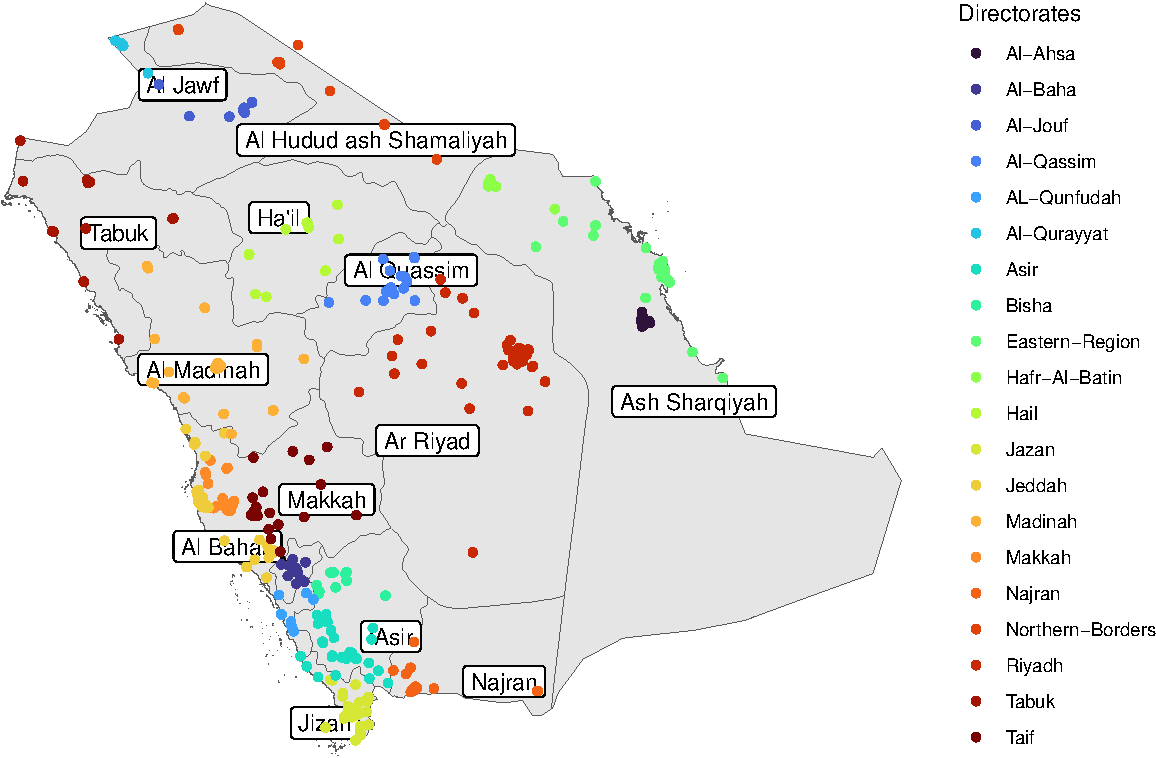
\includegraphics{lookups_files/figure-pdf/fig-scc-1.pdf}

}

\caption{\label{fig-scc}SCC location map with regional boundaries}

\end{figure}%

\begin{Shaded}
\begin{Highlighting}[]
\NormalTok{reg\_dir\_lu }\OtherTok{\textless{}{-}}\NormalTok{ sa\_bound }\SpecialCharTok{|\textgreater{}}
    \FunctionTok{st\_join}\NormalTok{(sc\_ll\_sf) }\SpecialCharTok{|\textgreater{}}
    \FunctionTok{st\_drop\_geometry}\NormalTok{() }\SpecialCharTok{|\textgreater{}}
    \FunctionTok{select}\NormalTok{(ADM1\_EN, name) }\SpecialCharTok{|\textgreater{}}
    \FunctionTok{group\_by}\NormalTok{(ADM1\_EN, name) }\SpecialCharTok{|\textgreater{}}
    \FunctionTok{summarise}\NormalTok{(}\AttributeTok{n =} \FunctionTok{n}\NormalTok{()) }\SpecialCharTok{|\textgreater{}}
    \FunctionTok{ungroup}\NormalTok{() }\SpecialCharTok{|\textgreater{}}
    \FunctionTok{group\_by}\NormalTok{(name) }\SpecialCharTok{|\textgreater{}}
    \FunctionTok{arrange}\NormalTok{(name) }\SpecialCharTok{|\textgreater{}}
    \FunctionTok{filter}\NormalTok{(n }\SpecialCharTok{==} \FunctionTok{max}\NormalTok{(n)) }\SpecialCharTok{|\textgreater{}}
    \FunctionTok{select}\NormalTok{(name, }\FunctionTok{everything}\NormalTok{())}
\end{Highlighting}
\end{Shaded}

Now we want to attach region names tpo the smoking data so we can join
with population data in order to calculate attendance rates by age.

\begin{Shaded}
\begin{Highlighting}[]
\NormalTok{pops}\SpecialCharTok{$}\NormalTok{Region }\SpecialCharTok{|\textgreater{}}
    \FunctionTok{unique}\NormalTok{() }\SpecialCharTok{|\textgreater{}}
    \FunctionTok{enframe}\NormalTok{() }
\end{Highlighting}
\end{Shaded}

\begin{verbatim}
# A tibble: 13 x 2
    name value                    
   <int> <chr>                    
 1     1 Al Bahah                 
 2     2 Al Jawf                  
 3     3 Al Hudud ash Shamaliyah  
 4     4 Ar Riyadh                
 5     5 Al Qasim                 
 6     6 Al Madinah al Munawwarah 
 7     7 Al Mintaqah ash Sharqiyah
 8     8 Tabuk                    
 9     9 Jazan                    
10    10 Ha'il                    
11    11 'Asir                    
12    12 Makkah al Mukarramah     
13    13 Najran                   
\end{verbatim}

\begin{Shaded}
\begin{Highlighting}[]
\NormalTok{smok\_1 }\OtherTok{\textless{}{-}}\NormalTok{ smok }\SpecialCharTok{|\textgreater{}}
    \FunctionTok{mutate}\NormalTok{(}\AttributeTok{directorate\_name =} \FunctionTok{recode}\NormalTok{(directorate\_name, }\StringTok{"Qurayyat"} \OtherTok{=} \StringTok{"Al{-}Qurayyat"}\NormalTok{, }
                                     \StringTok{"Qunfotha"} \OtherTok{=} \StringTok{"AL{-}Qunfudah"}\NormalTok{, }
                                     \StringTok{"AlAhsa"} \OtherTok{=} \StringTok{"Al{-}Ahsa"}\NormalTok{, }
                                     \StringTok{"Baha"} \OtherTok{=} \StringTok{"Al{-}Baha"}\NormalTok{,}
                                     \StringTok{"Eastern"} \OtherTok{=} \StringTok{"Eastern{-}Region"}\NormalTok{, }
                                     \StringTok{"Hafer AlBatin"} \OtherTok{=} \StringTok{"Hafr{-}Al{-}Batin"}\NormalTok{,}
                                     \StringTok{"Northern Borders"} \OtherTok{=} \StringTok{"Northern{-}Borders"}\NormalTok{,}
                                     \StringTok{"Qassim"} \OtherTok{=} \StringTok{"Al{-}Qassim"}\NormalTok{, }
                                     \StringTok{"Jouf"} \OtherTok{=} \StringTok{"Al{-}Jouf"}
\NormalTok{                                     )) }\SpecialCharTok{|\textgreater{}}
    \FunctionTok{left\_join}\NormalTok{(reg\_dir\_lu, }\AttributeTok{by =} \FunctionTok{c}\NormalTok{(}\StringTok{"directorate\_name"} \OtherTok{=} \StringTok{"name"}\NormalTok{)) }
    \CommentTok{\#left\_join(pops, by = c("ADM1\_EN" = "Region"))}
\end{Highlighting}
\end{Shaded}

\begin{Shaded}
\begin{Highlighting}[]
\NormalTok{pops }\OtherTok{\textless{}{-}}\NormalTok{ pops }\SpecialCharTok{|\textgreater{}}
    \FunctionTok{mutate}\NormalTok{(}\AttributeTok{age =} \FunctionTok{parse\_number}\NormalTok{(}\StringTok{\textasciigrave{}}\AttributeTok{Single Age Group}\StringTok{\textasciigrave{}}\NormalTok{))}

\NormalTok{pops}\SpecialCharTok{$}\NormalTok{Region }\SpecialCharTok{|\textgreater{}}
    \FunctionTok{unique}\NormalTok{()}
\end{Highlighting}
\end{Shaded}

\begin{verbatim}
 [1] "Al Bahah"                  "Al Jawf"                  
 [3] "Al Hudud ash Shamaliyah"   "Ar Riyadh"                
 [5] "Al Qasim"                  "Al Madinah al Munawwarah" 
 [7] "Al Mintaqah ash Sharqiyah" "Tabuk"                    
 [9] "Jazan"                     "Ha'il"                    
[11] "'Asir"                     "Makkah al Mukarramah"     
[13] "Najran"                   
\end{verbatim}

\begin{Shaded}
\begin{Highlighting}[]
\NormalTok{smok\_pops\_region }\OtherTok{\textless{}{-}}\NormalTok{ smok\_1 }\SpecialCharTok{|\textgreater{}}
    \FunctionTok{mutate}\NormalTok{(}\AttributeTok{Gender =} \FunctionTok{str\_to\_title}\NormalTok{(patient\_gender)) }\SpecialCharTok{|\textgreater{}}
    \FunctionTok{count}\NormalTok{(ADM1\_EN, age, Gender) }


\DocumentationTok{\#\# recode region names (ADM1\_EN)}

\CommentTok{\# smok\_pops\_region |\textgreater{}}
\CommentTok{\#     mutate(Region = recode(ADM1\_EN, }
\CommentTok{\#                            "\textasciigrave{}Asir" = "\textquotesingle{}Asir", }
\CommentTok{\#                            "Ash Sharqiyah" = "Al Hudud ash Sharqiyah", }
\CommentTok{\#                            "Al Madinah" = ))}

\NormalTok{smok\_pops\_region }\OtherTok{\textless{}{-}}\NormalTok{ smok\_pops\_region }\SpecialCharTok{|\textgreater{}}
    \FunctionTok{full\_join}\NormalTok{(pops, }\AttributeTok{by =} \FunctionTok{c}\NormalTok{(}\StringTok{"ADM1\_EN"} \OtherTok{=} \StringTok{"Region"}\NormalTok{, }\StringTok{"age"}\NormalTok{, }\StringTok{"Gender"}\NormalTok{)) }



\DocumentationTok{\#\# sense check}
\NormalTok{smok\_pops\_region }\SpecialCharTok{|\textgreater{}}
    \FunctionTok{count}\NormalTok{(Gender, ADM1\_EN, }\StringTok{\textasciigrave{}}\AttributeTok{18{-}44}\StringTok{\textasciigrave{}}\NormalTok{) }\SpecialCharTok{|\textgreater{}}
    \FunctionTok{print}\NormalTok{(}\AttributeTok{n =} \DecValTok{42}\NormalTok{)}
\end{Highlighting}
\end{Shaded}

\begin{verbatim}
# A tibble: 69 x 4
   Gender ADM1_EN                   `18-44`     n
   <chr>  <chr>                     <chr>   <int>
 1 Female 'Asir                     18-44     967
 2 Female 'Asir                     other    2206
 3 Female Al Bahah                  18-44     535
 4 Female Al Bahah                  other    1178
 5 Female Al Hudud ash Shamaliyah   18-44     216
 6 Female Al Hudud ash Shamaliyah   other     522
 7 Female Al Jawf                   18-44     216
 8 Female Al Jawf                   other     522
 9 Female Al Madinah                <NA>       17
10 Female Al Madinah al Munawwarah  18-44     484
11 Female Al Madinah al Munawwarah  other    1133
12 Female Al Mintaqah ash Sharqiyah 18-44     648
13 Female Al Mintaqah ash Sharqiyah other    1568
14 Female Al Qasim                  18-44     699
15 Female Al Qasim                  other    1592
16 Female Al Quassim                <NA>        4
17 Female Ar Riyad                  <NA>       21
18 Female Ar Riyadh                 18-44    1241
19 Female Ar Riyadh                 other    2866
20 Female Ash Sharqiyah             <NA>       19
21 Female Ha'il                     18-44     482
22 Female Ha'il                     other    1045
23 Female Jazan                     18-44     913
24 Female Jazan                     other    2270
25 Female Jizan                     <NA>        5
26 Female Makkah                    <NA>       23
27 Female Makkah al Mukarramah      18-44     917
28 Female Makkah al Mukarramah      other    2224
29 Female Najran                    18-44     372
30 Female Najran                    other     821
31 Female Tabuk                     18-44     376
32 Female Tabuk                     other     876
33 Female `Asir                     <NA>       14
34 Male   'Asir                     18-44     967
35 Male   'Asir                     other    2293
36 Male   Al Bahah                  18-44     539
37 Male   Al Bahah                  other    1228
38 Male   Al Hudud ash Shamaliyah   18-44     216
39 Male   Al Hudud ash Shamaliyah   other     520
40 Male   Al Jawf                   18-44     216
41 Male   Al Jawf                   other     531
42 Male   Al Jawf                   <NA>        1
# i 27 more rows
\end{verbatim}

\begin{Shaded}
\begin{Highlighting}[]
\DocumentationTok{\#\# 18{-}44 F}
\NormalTok{smok\_18\_44 }\OtherTok{\textless{}{-}}\NormalTok{ smok\_pops\_region }\SpecialCharTok{|\textgreater{}}
    \FunctionTok{filter}\NormalTok{(Gender }\SpecialCharTok{==} \StringTok{"Female"}\NormalTok{, }\StringTok{\textasciigrave{}}\AttributeTok{18{-}44}\StringTok{\textasciigrave{}} \SpecialCharTok{==} \StringTok{"18{-}44"}\NormalTok{) }\SpecialCharTok{|\textgreater{}}
    \FunctionTok{group\_by}\NormalTok{(ADM1\_EN) }\SpecialCharTok{|\textgreater{}}
    \FunctionTok{reframe}\NormalTok{(}\AttributeTok{n =} \FunctionTok{n}\NormalTok{(), }
            \AttributeTok{sum\_pop =} \FunctionTok{sum}\NormalTok{(Population), }
            \AttributeTok{rate\_100k =} \DecValTok{100000} \SpecialCharTok{*}\NormalTok{ n }\SpecialCharTok{/}\NormalTok{ sum\_pop)}

\NormalTok{    smok\_18\_44\_ci }\OtherTok{\textless{}{-}}\NormalTok{ PHEindicatormethods}\SpecialCharTok{::}\FunctionTok{phe\_rate}\NormalTok{(smok\_18\_44, n, sum\_pop, }\AttributeTok{multiplier =} \DecValTok{100000}\NormalTok{)}

\NormalTok{smok\_18\_44\_ci }\SpecialCharTok{|\textgreater{}}
    \FunctionTok{ggplot}\NormalTok{() }\SpecialCharTok{+}
    \FunctionTok{geom\_col}\NormalTok{(}\FunctionTok{aes}\NormalTok{(}\FunctionTok{reorder}\NormalTok{(ADM1\_EN, }\SpecialCharTok{{-}}\NormalTok{rate\_100k), rate\_100k), }\AttributeTok{fill =} \StringTok{"goldenrod"}\NormalTok{) }\SpecialCharTok{+}
    \FunctionTok{geom\_point}\NormalTok{(}\FunctionTok{aes}\NormalTok{(}\FunctionTok{reorder}\NormalTok{(ADM1\_EN, }\SpecialCharTok{{-}}\NormalTok{rate\_100k), rate\_100k, }\AttributeTok{colour =}\NormalTok{ n)) }\SpecialCharTok{+}
    \FunctionTok{geom\_linerange}\NormalTok{(}\FunctionTok{aes}\NormalTok{(}\AttributeTok{x =}\NormalTok{ ADM1\_EN, }\AttributeTok{ymin =}\NormalTok{ lowercl, }\AttributeTok{ymax =}\NormalTok{ uppercl)) }\SpecialCharTok{+}
    \FunctionTok{labs}\NormalTok{(}\AttributeTok{y =} \StringTok{""}\NormalTok{, }
         \AttributeTok{x =} \StringTok{"Region}
\StringTok{         "}\NormalTok{) }\SpecialCharTok{+}
    \FunctionTok{theme}\NormalTok{(}\AttributeTok{axis.text.x =} \FunctionTok{element\_text}\NormalTok{(}\AttributeTok{angle =} \DecValTok{45}\NormalTok{, }\AttributeTok{hjust =} \DecValTok{1}\NormalTok{))}
\end{Highlighting}
\end{Shaded}

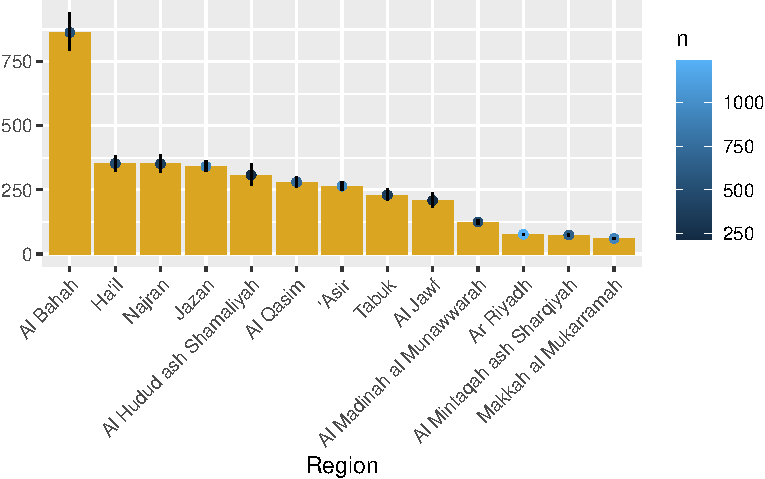
\includegraphics{lookups_files/figure-pdf/calculate smoking rates by region-1.pdf}

\begin{Shaded}
\begin{Highlighting}[]
\DocumentationTok{\#\# 15+}

\NormalTok{smok\_15\_ }\OtherTok{\textless{}{-}}\NormalTok{ smok\_pops\_region }\SpecialCharTok{|\textgreater{}}
    \FunctionTok{filter}\NormalTok{(}\StringTok{\textasciigrave{}}\AttributeTok{15+}\StringTok{\textasciigrave{}} \SpecialCharTok{==} \StringTok{"15+"}\NormalTok{) }\SpecialCharTok{|\textgreater{}}
    \FunctionTok{group\_by}\NormalTok{(ADM1\_EN) }\SpecialCharTok{|\textgreater{}}
    \FunctionTok{reframe}\NormalTok{(}\AttributeTok{n =} \FunctionTok{n}\NormalTok{(), }
            \AttributeTok{sum\_pop =} \FunctionTok{sum}\NormalTok{(Population), }
            \AttributeTok{rate\_100k =} \DecValTok{100000} \SpecialCharTok{*}\NormalTok{ n }\SpecialCharTok{/}\NormalTok{ sum\_pop)}

\NormalTok{smok\_15\_ci }\OtherTok{\textless{}{-}}\NormalTok{ PHEindicatormethods}\SpecialCharTok{::}\FunctionTok{phe\_rate}\NormalTok{(smok\_15\_, n, sum\_pop,  }\AttributeTok{multiplier =} \DecValTok{100000}\NormalTok{)}

\NormalTok{smok\_15\_ci }\SpecialCharTok{|\textgreater{}}
    \FunctionTok{ggplot}\NormalTok{() }\SpecialCharTok{+}
    \FunctionTok{geom\_point}\NormalTok{(}\FunctionTok{aes}\NormalTok{(}\FunctionTok{reorder}\NormalTok{(ADM1\_EN, rate\_100k), rate\_100k)) }\SpecialCharTok{+}
    \FunctionTok{geom\_linerange}\NormalTok{(}\FunctionTok{aes}\NormalTok{(}\AttributeTok{x =}\NormalTok{ ADM1\_EN, }\AttributeTok{ymin =}\NormalTok{ lowercl, }\AttributeTok{ymax =}\NormalTok{ uppercl)) }\SpecialCharTok{+}
    \FunctionTok{coord\_flip}\NormalTok{() }\SpecialCharTok{+}
    \FunctionTok{labs}\NormalTok{(}\AttributeTok{x =} \StringTok{""}\NormalTok{)}
\end{Highlighting}
\end{Shaded}

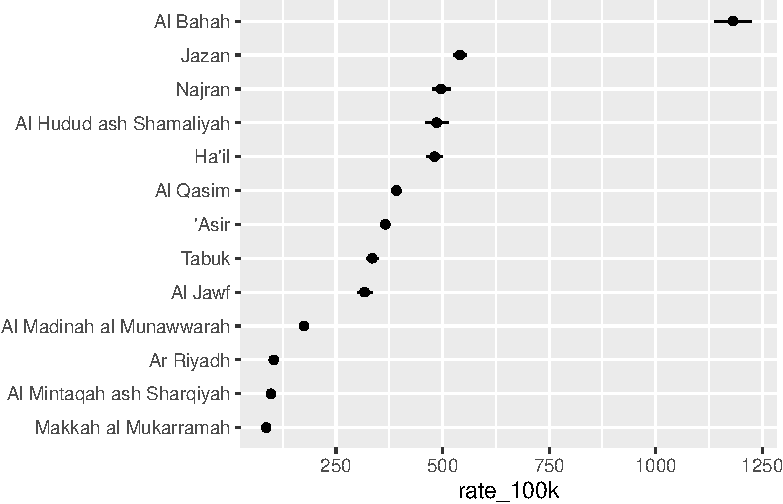
\includegraphics{lookups_files/figure-pdf/calculate smoking rates by region-2.pdf}

\begin{Shaded}
\begin{Highlighting}[]
\DocumentationTok{\#\# AS specific}

\NormalTok{smok\_pops\_region }\SpecialCharTok{|\textgreater{}}
    \CommentTok{\#filter(\textasciigrave{}15+\textasciigrave{} == "15+") |\textgreater{}}
    \FunctionTok{group\_by}\NormalTok{(ADM1\_EN, }\StringTok{\textasciigrave{}}\AttributeTok{Five{-}Year Age Group}\StringTok{\textasciigrave{}}\NormalTok{, Gender) }\SpecialCharTok{|\textgreater{}}
    \FunctionTok{reframe}\NormalTok{(}\AttributeTok{n =} \FunctionTok{n}\NormalTok{(), }
            \AttributeTok{sum\_pop =} \FunctionTok{sum}\NormalTok{(Population), }
            \AttributeTok{rate\_100k =} \DecValTok{100} \SpecialCharTok{*}\NormalTok{ n }\SpecialCharTok{/}\NormalTok{ sum\_pop) }\SpecialCharTok{|\textgreater{}}
   \CommentTok{\# select({-}c(n, sum\_pop)) |\textgreater{}}
    \FunctionTok{pivot\_wider}\NormalTok{(}\SpecialCharTok{{-}}\FunctionTok{c}\NormalTok{(n, rate\_100k), }\AttributeTok{names\_from =} \FunctionTok{c}\NormalTok{(}\StringTok{"Gender"}\NormalTok{, }\StringTok{"Five{-}Year Age Group"}\NormalTok{), }\AttributeTok{values\_from =} \StringTok{"sum\_pop"}\NormalTok{) }
\end{Highlighting}
\end{Shaded}

\begin{verbatim}
# A tibble: 20 x 38
   ADM1_EN    `Female_0-4` `Male_0-4` `Female_10-14` `Male_10-14` `Female_15-19`
   <chr>             <int>      <int>          <int>        <int>          <int>
 1 'Asir             86076      89700          89842        92719          80089
 2 Al Bahah          13905      14292          15738        16437          13866
 3 Al Hudud ~        20196      21493          17737        18266          14648
 4 Al Jawf           35470      36359          29566        30401          23021
 5 Al Madinah           NA         NA             NA           NA             NA
 6 Al Madina~        92536      95669          91346        94512          78252
 7 Al Mintaq~       200425     208376         184743       191018         149977
 8 Al Qasim          54714      56834          57093        58495          50842
 9 Al Quassim           NA         NA             NA           NA             NA
10 Ar Riyad             NA         NA             NA           NA             NA
11 Ar Riyadh        307991     320698         298933       309250         254888
12 Ash Sharq~           NA         NA             NA           NA             NA
13 Ha'il             32737      33782          32674        33511          27449
14 Jazan             64626      67613          64993        68873          59475
15 Jizan                NA         NA             NA           NA             NA
16 Makkah               NA         NA             NA           NA             NA
17 Makkah al~       281082     292376         299840       314392         270382
18 Najran            31863      33038          27125        28865          22482
19 Tabuk             42296      44012          39399        40646          34513
20 `Asir                NA         NA             NA           NA             NA
# i 32 more variables: `Male_15-19` <int>, `Female_20-24` <int>,
#   `Male_20-24` <int>, `Female_25-29` <int>, `Male_25-29` <int>,
#   `Female_30-34` <int>, `Male_30-34` <int>, `Female_35-39` <int>,
#   `Male_35-39` <int>, `Female_40-44` <int>, `Male_40-44` <int>,
#   `Female_45-49` <int>, `Male_45-49` <int>, `Female_5-9` <int>,
#   `Male_5-9` <int>, `Female_50-54` <int>, `Male_50-54` <int>,
#   `Female_55-59` <int>, `Male_55-59` <int>, `Female_60-64` <int>, ...
\end{verbatim}

\bookmarksetup{startatroot}

\chapter{AMR walkthrough}\label{amr-walkthrough}

\bookmarksetup{startatroot}

\chapter{Introduction}\label{introduction-1}

This document outlines a stepwise approach to calculating AMR indicators
from dummy data kindly supplied by PHA.

There are x steps

\begin{enumerate}
\def\labelenumi{\arabic{enumi}.}
\item
  EDA (exploratory data analysis of raw data) - this involves cleaning,
  visualisation and creation of relevant variables.
\item
  Review of indicator definitions

  \begin{itemize}
  \item
    Numerator
  \item
    Denominator
  \end{itemize}
\item
  Method for calculating numerator and denominator values from dataset.
  The outline uses R code for reproducibility and flexibility.
\item
  Calculating indicator values and uncertainty intervals
\item
  Suggested indicator visualisations (if appropriate).
\end{enumerate}

\bookmarksetup{startatroot}

\chapter{AMR indicators}\label{amr-indicators}

\subsection{MRSA}\label{mrsa}

\begin{quote}
Percentage of bloodstream infection due to methicillin-resistant
Staphylococcus aureus (MRSA)
\end{quote}

\begin{quote}
Numerator: No.~of patients with growth of methicillin-resistant S.
aureus in tested blood samples
\end{quote}

\begin{quote}
Denominator: Total No.~of patients with growth of S. aureus in tested
blood samples
\end{quote}

\subsection{E. coli}\label{e.-coli}

\begin{quote}
Percentage of bloodstream infection due to 3rd-generation cephalosporin
resistant E. coli
\end{quote}

\begin{quote}
Numerator: No.~of patients with growth of 3rd-generation cephalosporin
resistant E. coli in tested blood samples
\end{quote}

\begin{quote}
Denominator: Total No.~of patients with growth of E. coli in tested
blood samples
\end{quote}

\subsection{Import data}\label{import-data}

\begin{Shaded}
\begin{Highlighting}[]
\NormalTok{df }\OtherTok{\textless{}{-}}\NormalTok{ amr}
\end{Highlighting}
\end{Shaded}

334 observations

\section{Data preparation}\label{data-preparation}

\subsection{calculate 5-year age
bands}\label{calculate-5-year-age-bands}

\begin{Shaded}
\begin{Highlighting}[]
\NormalTok{amr }\OtherTok{\textless{}{-}}\NormalTok{ amr[, }\StringTok{\textasciigrave{}}\AttributeTok{:=}\StringTok{\textasciigrave{}}\NormalTok{ (}\AttributeTok{five\_year =} \FunctionTok{cut}\NormalTok{(age\_year, }\AttributeTok{breaks =} \FunctionTok{seq}\NormalTok{(}\DecValTok{0}\NormalTok{, }\DecValTok{100}\NormalTok{, }\DecValTok{5}\NormalTok{), }\AttributeTok{right =} \ConstantTok{FALSE}\NormalTok{))][]}

\FunctionTok{head}\NormalTok{(amr)}
\end{Highlighting}
\end{Shaded}

\begin{verbatim}
   record_number sample_no patient_mrn   location
           <num>    <char>      <char>     <char>
1:             1    ######       ##### Outpatient
2:            17    ######       #####  Inpatient
3:            20    ######       #####  Inpatient
4:            25    ######       #####  Inpatient
5:            43    ######       ##### Outpatient
6:            63    ######       ##### Outpatient
                                                     patient_hospitalized
                                                                   <char>
1: Patient had NOT been admitted for more than 2 days in the past 30 days
2:                       Patient has been hospitalized for 2 days or less
3:                     Patient has been hospitalized for more than 2 days
4:                       Patient has been hospitalized for 2 days or less
5: Patient had NOT been admitted for more than 2 days in the past 30 days
6: Patient had NOT been admitted for more than 2 days in the past 30 days
     specific_location age_year community_origin   site first_name second_name
                <char>    <num>           <char> <char>     <char>      <char>
1:      Emergency Room        0 Community Origin  Blood       ####       #####
2: Intensive Care Unit       71 Community Origin  Blood       ####       #####
3: Intensive Care Unit       44  Hospital Origin  Blood       ####       #####
4: Intensive Care Unit       67 Community Origin  Blood       ####       #####
5:      Emergency Room       67 Community Origin  Blood       ####       #####
6:      Emergency Room       92 Community Origin  Blood       ####       #####
   family_name national_iqama_id nationality    pathogen_name minocycline
        <char>            <char>      <char>           <char>      <lgcl>
1:        ####        ##########       ##### Escherichia coli          NA
2:        ####        ##########       ##### Escherichia coli          NA
3:        ####        ##########       ##### Escherichia coli          NA
4:        ####        ##########       ##### Escherichia coli          NA
5:        ####        ##########       ##### Escherichia coli          NA
6:        ####        ##########       ##### Escherichia coli          NA
   tigecycline ampicillin penicillin_g oxacillin cefoxitin cefotaxime
        <lgcl>     <char>       <lgcl>    <char>    <char>     <char>
1:          NA          R           NA      <NA>      <NA>          R
2:          NA          R           NA      <NA>      <NA>         NA
3:          NA          S           NA      <NA>      <NA>          S
4:          NA          R           NA      <NA>      <NA>          R
5:          NA          R           NA      <NA>      <NA>         NA
6:          NA          R           NA      <NA>      <NA>         NA
   ceftazidime ceftriaxone cefixime cefepime doripenem ertapenem imipenem
        <char>      <char>   <lgcl>   <char>    <char>    <char>   <char>
1:           R           R       NA        R        NA         S        S
2:           S           S       NA        S        NA         S        S
3:           S           S       NA        S        NA         S        S
4:           R           R       NA        R        NA         S        S
5:           I           S       NA        S        NA         S        S
6:           R           R       NA        R         R         S        S
   meropenem co_trimoxazole azithromycin amikacin gentamicin ciprofloxacin
      <char>         <char>       <lgcl>   <lgcl>     <lgcl>        <char>
1:         S              S           NA       NA         NA             S
2:         S              S           NA       NA         NA             S
3:         S              S           NA       NA         NA             S
4:         S              R           NA       NA         NA             S
5:         S              S           NA       NA         NA             S
6:         S              R           NA       NA         NA             R
   levofloxacin colistin spectinomycin five_year
         <char>   <char>        <lgcl>    <fctr>
1:            S       NA            NA     [0,5)
2:            S        S            NA   [70,75)
3:            S       NA            NA   [40,45)
4:            S       NA            NA   [65,70)
5:            S        S            NA   [65,70)
6:            R        S            NA   [90,95)
\end{verbatim}

\subsection{remove non-relevant data}\label{remove-non-relevant-data}

This step removes identifiers (names, record IDs)

\begin{Shaded}
\begin{Highlighting}[]
\NormalTok{amr }\OtherTok{\textless{}{-}}\NormalTok{ amr }\SpecialCharTok{|\textgreater{}} \FunctionTok{select}\NormalTok{(}\SpecialCharTok{{-}}\FunctionTok{c}\NormalTok{(family\_name, first\_name, sample\_no, patient\_mrn, second\_name, national\_iqama\_id, nationality))}
\end{Highlighting}
\end{Shaded}

\subsection{create per test file (long
data)}\label{create-per-test-file-long-data}

\begin{itemize}
\tightlist
\item
  this create a \emph{per test} dataset rather than a per patient sample
  dataset
\end{itemize}

\begin{Shaded}
\begin{Highlighting}[]
\NormalTok{amr\_long }\OtherTok{\textless{}{-}}\NormalTok{ amr }\SpecialCharTok{|\textgreater{}}
    \FunctionTok{pivot\_longer}\NormalTok{(}\AttributeTok{names\_to =} \StringTok{"antibiotic\_test"}\NormalTok{, }\AttributeTok{values\_to =} \StringTok{"resistance"}\NormalTok{, }\AttributeTok{cols =}\NormalTok{ minocycline}\SpecialCharTok{:}\NormalTok{spectinomycin) }\SpecialCharTok{|\textgreater{}} \FunctionTok{setDT}\NormalTok{()}
\end{Highlighting}
\end{Shaded}

\subsection{recode 3rd generation
cephalosporins}\label{recode-3rd-generation-cephalosporins}

\begin{itemize}
\tightlist
\item
  this step adds a new variable which labels 3rd generation
  cephalosporins
\end{itemize}

\begin{Shaded}
\begin{Highlighting}[]
\NormalTok{amr\_long }\OtherTok{\textless{}{-}}\NormalTok{ amr\_long[, gen\_3 }\SpecialCharTok{:}\ErrorTok{=} \FunctionTok{case\_when}\NormalTok{(}\FunctionTok{str\_detect}\NormalTok{(antibiotic\_test, }\StringTok{"cef"}\NormalTok{) }\SpecialCharTok{\textasciitilde{}} \StringTok{"3rd{-}gen"}\NormalTok{, }\ConstantTok{TRUE} \SpecialCharTok{\textasciitilde{}} \StringTok{"other"}\NormalTok{)][]}
\end{Highlighting}
\end{Shaded}

\section{Data summarisation and description
(EDA)}\label{data-summarisation-and-description-eda}

\begin{itemize}
\tightlist
\item
  first generate a high level tabular summary
\end{itemize}

\begin{Shaded}
\begin{Highlighting}[]
\NormalTok{gtsummary}\SpecialCharTok{::}\FunctionTok{tbl\_summary}\NormalTok{(amr)}
\end{Highlighting}
\end{Shaded}

\begin{itemize}
\tightlist
\item
  represent this visually - we'll use decompostion trees
\end{itemize}

\begin{Shaded}
\begin{Highlighting}[]
\NormalTok{amr\_freq }\OtherTok{\textless{}{-}}\NormalTok{ amr\_long[pathogen\_name }\SpecialCharTok{==} \StringTok{"Escherichia coli"}\NormalTok{, .N, by }\OtherTok{=}\NormalTok{ .(five\_year, gen\_3, resistance, pathogen\_name)]}

\FunctionTok{collapsibleTreeSummary}\NormalTok{(amr\_freq, }
                       \FunctionTok{c}\NormalTok{(}\StringTok{"gen\_3"}\NormalTok{, }\StringTok{"resistance"}\NormalTok{), }
                       \AttributeTok{root =} \StringTok{"E. coli"}\NormalTok{, }
                       \AttributeTok{nodeSize =} \StringTok{"N"}\NormalTok{, }
                       \AttributeTok{attribute =} \StringTok{"N"}\NormalTok{, }
                       \AttributeTok{fontSize =} \DecValTok{16}\NormalTok{, }
                       \AttributeTok{collapsed =} \ConstantTok{FALSE}\NormalTok{)}
\end{Highlighting}
\end{Shaded}

\section{Numerators and denominators}\label{numerators-and-denominators}

\begin{itemize}
\tightlist
\item
  to calculate indicators we need to calculate
\item
  patients with blood stream infection
\item
  samples with antibiotic resistance
\end{itemize}

\begin{Shaded}
\begin{Highlighting}[]
\NormalTok{amr\_long}
\end{Highlighting}
\end{Shaded}

\begin{verbatim}
      record_number   location
              <num>     <char>
   1:             1 Outpatient
   2:             1 Outpatient
   3:             1 Outpatient
   4:             1 Outpatient
   5:             1 Outpatient
  ---                         
7678:          1210  Inpatient
7679:          1210  Inpatient
7680:          1210  Inpatient
7681:          1210  Inpatient
7682:          1210  Inpatient
                                                        patient_hospitalized
                                                                      <char>
   1: Patient had NOT been admitted for more than 2 days in the past 30 days
   2: Patient had NOT been admitted for more than 2 days in the past 30 days
   3: Patient had NOT been admitted for more than 2 days in the past 30 days
   4: Patient had NOT been admitted for more than 2 days in the past 30 days
   5: Patient had NOT been admitted for more than 2 days in the past 30 days
  ---                                                                       
7678:                     Patient has been hospitalized for more than 2 days
7679:                     Patient has been hospitalized for more than 2 days
7680:                     Patient has been hospitalized for more than 2 days
7681:                     Patient has been hospitalized for more than 2 days
7682:                     Patient has been hospitalized for more than 2 days
       specific_location age_year community_origin   site         pathogen_name
                  <char>    <num>           <char> <char>                <char>
   1:     Emergency Room        0 Community Origin  Blood      Escherichia coli
   2:     Emergency Room        0 Community Origin  Blood      Escherichia coli
   3:     Emergency Room        0 Community Origin  Blood      Escherichia coli
   4:     Emergency Room        0 Community Origin  Blood      Escherichia coli
   5:     Emergency Room        0 Community Origin  Blood      Escherichia coli
  ---                                                                          
7678: Non Intensive Unit       96  Hospital Origin  Blood Staphylococcus aureus
7679: Non Intensive Unit       96  Hospital Origin  Blood Staphylococcus aureus
7680: Non Intensive Unit       96  Hospital Origin  Blood Staphylococcus aureus
7681: Non Intensive Unit       96  Hospital Origin  Blood Staphylococcus aureus
7682: Non Intensive Unit       96  Hospital Origin  Blood Staphylococcus aureus
      five_year antibiotic_test resistance  gen_3
         <fctr>          <char>     <char> <char>
   1:     [0,5)     minocycline       <NA>  other
   2:     [0,5)     tigecycline       <NA>  other
   3:     [0,5)      ampicillin          R  other
   4:     [0,5)    penicillin_g       <NA>  other
   5:     [0,5)       oxacillin       <NA>  other
  ---                                            
7678:  [95,100)      gentamicin       <NA>  other
7679:  [95,100)   ciprofloxacin          R  other
7680:  [95,100)    levofloxacin          R  other
7681:  [95,100)        colistin         NA  other
7682:  [95,100)   spectinomycin       <NA>  other
\end{verbatim}

\section{Calculate resistance rates}\label{calculate-resistance-rates}

\begin{itemize}
\tightlist
\item
  calculate proportion of tests resistant
\item
  calculate confidence interval (using Wilsons score method for
  proportions via the \texttt{PHEindicatormethods} R package)
\end{itemize}

\begin{Shaded}
\begin{Highlighting}[]
\NormalTok{amr\_long[pathogen\_name }\SpecialCharTok{==} \StringTok{"Staphylococcus aureus"} \SpecialCharTok{\&} \SpecialCharTok{!}\FunctionTok{is.na}\NormalTok{(resistance), .N, by }\OtherTok{=}\NormalTok{ .(resistance)] }\SpecialCharTok{|\textgreater{}}
    \FunctionTok{pivot\_wider}\NormalTok{(}\AttributeTok{names\_from =}\NormalTok{ resistance, }\AttributeTok{values\_from =}\NormalTok{ N) }\SpecialCharTok{|\textgreater{}}
    \FunctionTok{rowwise}\NormalTok{() }\SpecialCharTok{|\textgreater{}}
    \FunctionTok{mutate}\NormalTok{(}\AttributeTok{total\_tests =} \FunctionTok{sum}\NormalTok{(}\FunctionTok{c\_across}\NormalTok{(S}\SpecialCharTok{:}\NormalTok{I), }\AttributeTok{na.rm =} \ConstantTok{TRUE}\NormalTok{), }
           \AttributeTok{resistance\_rate =}\NormalTok{ R }\SpecialCharTok{/}\NormalTok{ total\_tests)}
\end{Highlighting}
\end{Shaded}

\begin{verbatim}
# A tibble: 1 x 6
# Rowwise: 
      S  `NA`     R     I total_tests resistance_rate
  <int> <int> <int> <int>       <int>           <dbl>
1   947   281   545    11        1784           0.305
\end{verbatim}

by antibiotic

\begin{Shaded}
\begin{Highlighting}[]
\FunctionTok{options}\NormalTok{(}\AttributeTok{digits =} \DecValTok{2}\NormalTok{)}

\NormalTok{amr\_res\_ci\_sa }\OtherTok{\textless{}{-}}\NormalTok{ amr\_long[pathogen\_name }\SpecialCharTok{==} \StringTok{"Staphylococcus aureus"} \SpecialCharTok{\&} \SpecialCharTok{!}\FunctionTok{is.na}\NormalTok{(resistance), .N, by }\OtherTok{=}\NormalTok{ .(antibiotic\_test, resistance)] }\SpecialCharTok{|\textgreater{}}
    \FunctionTok{pivot\_wider}\NormalTok{(}\AttributeTok{names\_from =}\NormalTok{ resistance, }\AttributeTok{values\_from =}\NormalTok{ N, }\AttributeTok{values\_fill =} \DecValTok{0}\NormalTok{) }\SpecialCharTok{|\textgreater{}}
    \FunctionTok{rowwise}\NormalTok{() }\SpecialCharTok{|\textgreater{}}
    \FunctionTok{mutate}\NormalTok{(}\AttributeTok{total\_tests =} \FunctionTok{sum}\NormalTok{(}\FunctionTok{c\_across}\NormalTok{(S}\SpecialCharTok{:}\NormalTok{I), }\AttributeTok{na.rm =} \ConstantTok{TRUE}\NormalTok{), }
           \AttributeTok{resistance\_rate =}\NormalTok{ R }\SpecialCharTok{/}\NormalTok{ total\_tests)}

\FunctionTok{phe\_proportion}\NormalTok{(amr\_res\_ci\_sa, R, total\_tests) }\SpecialCharTok{|\textgreater{}}
    \FunctionTok{bind\_cols}\NormalTok{(amr\_res\_ci\_sa) }\SpecialCharTok{|\textgreater{}}
    \FunctionTok{ggplot}\NormalTok{() }\SpecialCharTok{+}
    \FunctionTok{geom\_point}\NormalTok{(}\FunctionTok{aes}\NormalTok{(}\FunctionTok{reorder}\NormalTok{(antibiotic\_test, value), value)) }\SpecialCharTok{+}
    \FunctionTok{geom\_linerange}\NormalTok{(}\FunctionTok{aes}\NormalTok{(antibiotic\_test, }\AttributeTok{ymin =}\NormalTok{ lowercl, }\AttributeTok{ymax =}\NormalTok{ uppercl)) }\SpecialCharTok{+}
    \FunctionTok{coord\_flip}\NormalTok{() }\SpecialCharTok{+}
    \FunctionTok{labs}\NormalTok{(}\AttributeTok{y =} \StringTok{"Staph. aureus resistance rate"}\NormalTok{, }\AttributeTok{x =} \StringTok{""}\NormalTok{) }\SpecialCharTok{+} 
    \FunctionTok{scale\_y\_continuous}\NormalTok{(}\AttributeTok{position =} \StringTok{"right"}\NormalTok{)}
\end{Highlighting}
\end{Shaded}

\begin{verbatim}
New names:
* `R` -> `R...1`
* `total_tests` -> `total_tests...2`
* `R` -> `R...12`
* `total_tests` -> `total_tests...14`
\end{verbatim}

\includegraphics{amr_poc_files/figure-pdf/unnamed-chunk-11-1.pdf}

by age

\begin{Shaded}
\begin{Highlighting}[]
\NormalTok{amr\_res\_ci\_age }\OtherTok{\textless{}{-}}\NormalTok{ amr\_long[pathogen\_name }\SpecialCharTok{==} \StringTok{"Staphylococcus aureus"} \SpecialCharTok{\&} \SpecialCharTok{!}\FunctionTok{is.na}\NormalTok{(resistance), .N, by }\OtherTok{=}\NormalTok{ .(five\_year, resistance)] }\SpecialCharTok{|\textgreater{}}
    \FunctionTok{pivot\_wider}\NormalTok{(}\AttributeTok{names\_from =}\NormalTok{ resistance, }\AttributeTok{values\_from =}\NormalTok{ N, }\AttributeTok{values\_fill =} \DecValTok{0}\NormalTok{) }\SpecialCharTok{|\textgreater{}}
    \FunctionTok{rowwise}\NormalTok{() }\SpecialCharTok{|\textgreater{}}
    \FunctionTok{mutate}\NormalTok{(}\AttributeTok{total\_tests =} \FunctionTok{sum}\NormalTok{(}\FunctionTok{c\_across}\NormalTok{(S}\SpecialCharTok{:}\NormalTok{I), }\AttributeTok{na.rm =} \ConstantTok{TRUE}\NormalTok{), }
           \AttributeTok{resistance\_rate =}\NormalTok{ R }\SpecialCharTok{/}\NormalTok{ total\_tests)}

\FunctionTok{phe\_proportion}\NormalTok{(amr\_res\_ci\_age, R, total\_tests) }\SpecialCharTok{|\textgreater{}}
    \FunctionTok{bind\_cols}\NormalTok{(amr\_res\_ci\_age) }\SpecialCharTok{|\textgreater{}}
    \FunctionTok{ggplot}\NormalTok{() }\SpecialCharTok{+}
    \FunctionTok{geom\_point}\NormalTok{(}\FunctionTok{aes}\NormalTok{(}\FunctionTok{reorder}\NormalTok{(five\_year, value), value)) }\SpecialCharTok{+}
    \FunctionTok{geom\_linerange}\NormalTok{(}\FunctionTok{aes}\NormalTok{(five\_year, }\AttributeTok{ymin =}\NormalTok{ lowercl, }\AttributeTok{ymax =}\NormalTok{ uppercl)) }\SpecialCharTok{+}
    \FunctionTok{coord\_flip}\NormalTok{() }\SpecialCharTok{+}
    \FunctionTok{labs}\NormalTok{(}\AttributeTok{y =} \StringTok{"Staph. aureus resistance rate"}\NormalTok{, }\AttributeTok{x =} \StringTok{""}\NormalTok{) }\SpecialCharTok{+} 
    \FunctionTok{scale\_y\_continuous}\NormalTok{(}\AttributeTok{position =} \StringTok{"right"}\NormalTok{)}
\end{Highlighting}
\end{Shaded}

\begin{verbatim}
New names:
* `R` -> `R...1`
* `total_tests` -> `total_tests...2`
* `R` -> `R...12`
* `total_tests` -> `total_tests...14`
\end{verbatim}

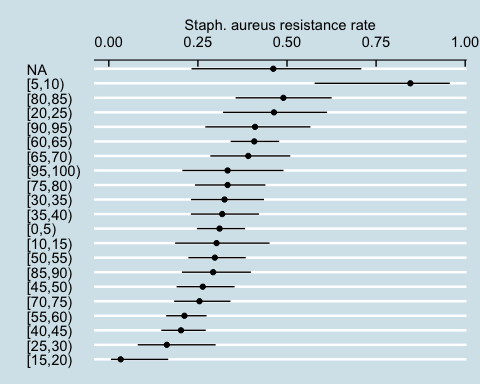
\includegraphics{amr_poc_files/figure-pdf/by age-1.pdf}

\section{E. coli}\label{e.-coli-1}

\begin{Shaded}
\begin{Highlighting}[]
\NormalTok{amr\_res\_ci\_ec }\OtherTok{\textless{}{-}}\NormalTok{ amr\_long[}\FunctionTok{str\_detect}\NormalTok{(pathogen\_name, }\StringTok{"coli"}\NormalTok{) }\SpecialCharTok{\&} \SpecialCharTok{!}\FunctionTok{is.na}\NormalTok{(resistance), .N, by }\OtherTok{=}\NormalTok{ .(antibiotic\_test, resistance, gen\_3)] }\SpecialCharTok{|\textgreater{}}
    \FunctionTok{pivot\_wider}\NormalTok{(}\AttributeTok{names\_from =}\NormalTok{ resistance, }\AttributeTok{values\_from =}\NormalTok{ N, }\AttributeTok{values\_fill =} \DecValTok{0}\NormalTok{) }\SpecialCharTok{|\textgreater{}}
    \FunctionTok{rowwise}\NormalTok{() }\SpecialCharTok{|\textgreater{}}
    \FunctionTok{mutate}\NormalTok{(}\AttributeTok{total\_tests =} \FunctionTok{sum}\NormalTok{(}\FunctionTok{c\_across}\NormalTok{(R}\SpecialCharTok{:}\NormalTok{I), }\AttributeTok{na.rm =} \ConstantTok{TRUE}\NormalTok{), }
           \AttributeTok{resistance\_rate =}\NormalTok{ R }\SpecialCharTok{/}\NormalTok{ total\_tests)}

\FunctionTok{phe\_proportion}\NormalTok{(amr\_res\_ci\_ec, R, total\_tests) }\SpecialCharTok{|\textgreater{}}
    \FunctionTok{bind\_cols}\NormalTok{(amr\_res\_ci\_ec) }\SpecialCharTok{|\textgreater{}}
    \FunctionTok{ggplot}\NormalTok{() }\SpecialCharTok{+}
    \FunctionTok{geom\_point}\NormalTok{(}\FunctionTok{aes}\NormalTok{(}\FunctionTok{reorder}\NormalTok{(antibiotic\_test, value), value, }\AttributeTok{colour =}\NormalTok{ gen\_3)) }\SpecialCharTok{+}
    \FunctionTok{geom\_linerange}\NormalTok{(}\FunctionTok{aes}\NormalTok{(antibiotic\_test, }\AttributeTok{ymin =}\NormalTok{ lowercl, }\AttributeTok{ymax =}\NormalTok{ uppercl)) }\SpecialCharTok{+}
    \FunctionTok{coord\_flip}\NormalTok{() }\SpecialCharTok{+}
    \FunctionTok{labs}\NormalTok{(}\AttributeTok{y =} \StringTok{"E. coli resistance rate"}\NormalTok{, }\AttributeTok{x =} \StringTok{""}\NormalTok{) }\SpecialCharTok{+} \FunctionTok{scale\_y\_continuous}\NormalTok{(}\AttributeTok{position =} \StringTok{"right"}\NormalTok{)}
\end{Highlighting}
\end{Shaded}

\begin{verbatim}
New names:
* `R` -> `R...1`
* `total_tests` -> `total_tests...2`
* `R` -> `R...11`
* `total_tests` -> `total_tests...15`
\end{verbatim}

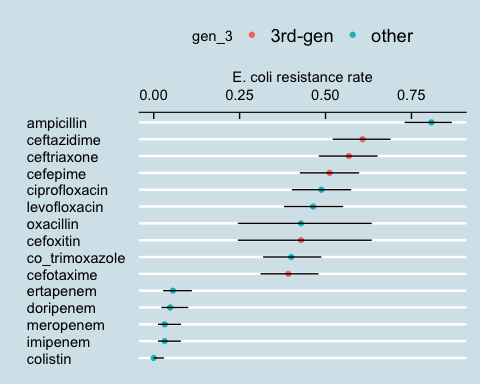
\includegraphics{amr_poc_files/figure-pdf/e coli-1.pdf}

\subsubsection{select methicillin tested
samples}\label{select-methicillin-tested-samples}

\begin{Shaded}
\begin{Highlighting}[]
\NormalTok{amr[, .SD, .SDcols }\OtherTok{=} \FunctionTok{c}\NormalTok{(}\StringTok{"record\_number"}\NormalTok{, }\StringTok{"location"}\NormalTok{, }\StringTok{"patient\_hospitalized"}\NormalTok{, }\StringTok{"specific\_location"}\NormalTok{, }\StringTok{"community\_origin"}\NormalTok{, }\StringTok{"site"}\NormalTok{, }\StringTok{"pathogen\_name"}\NormalTok{, }\StringTok{"five\_year"}\NormalTok{)]}
\end{Highlighting}
\end{Shaded}

\begin{verbatim}
     record_number   location
             <num>     <char>
  1:             1 Outpatient
  2:            17  Inpatient
  3:            20  Inpatient
  4:            25  Inpatient
  5:            43 Outpatient
 ---                         
330:          1218  Inpatient
331:          1159 Outpatient
332:          1183 Outpatient
333:          1160 Outpatient
334:          1210  Inpatient
                                                       patient_hospitalized
                                                                     <char>
  1: Patient had NOT been admitted for more than 2 days in the past 30 days
  2:                       Patient has been hospitalized for 2 days or less
  3:                     Patient has been hospitalized for more than 2 days
  4:                       Patient has been hospitalized for 2 days or less
  5: Patient had NOT been admitted for more than 2 days in the past 30 days
 ---                                                                       
330:                       Patient has been hospitalized for 2 days or less
331: Patient had NOT been admitted for more than 2 days in the past 30 days
332: Patient had NOT been admitted for more than 2 days in the past 30 days
333: Patient had NOT been admitted for more than 2 days in the past 30 days
334:                     Patient has been hospitalized for more than 2 days
          specific_location community_origin   site         pathogen_name
                     <char>           <char> <char>                <char>
  1:         Emergency Room Community Origin  Blood      Escherichia coli
  2:    Intensive Care Unit Community Origin  Blood      Escherichia coli
  3:    Intensive Care Unit  Hospital Origin  Blood      Escherichia coli
  4:    Intensive Care Unit Community Origin  Blood      Escherichia coli
  5:         Emergency Room Community Origin  Blood      Escherichia coli
 ---                                                                     
330:     Non Intensive Unit Community Origin  Blood      Escherichia coli
331:         Emergency Room Community Origin  Blood Staphylococcus aureus
332: Out Patient Department Community Origin  Blood Staphylococcus aureus
333:         Emergency Room Community Origin  Blood      Escherichia coli
334:     Non Intensive Unit  Hospital Origin  Blood Staphylococcus aureus
     five_year
        <fctr>
  1:     [0,5)
  2:   [70,75)
  3:   [40,45)
  4:   [65,70)
  5:   [65,70)
 ---          
330:   [80,85)
331:   [85,90)
332:   [85,90)
333:   [90,95)
334:  [95,100)
\end{verbatim}

\bookmarksetup{startatroot}

\chapter{smoking-poc}\label{smoking-poc}

\section{}\label{section}

\subsection{Data preparation}\label{data-preparation-1}

\begin{Shaded}
\begin{Highlighting}[]
\NormalTok{smoking }\OtherTok{\textless{}{-}}\NormalTok{ smoking[, }\StringTok{\textasciigrave{}}\AttributeTok{:=}\StringTok{\textasciigrave{}}\NormalTok{ (}\AttributeTok{five\_year =} \FunctionTok{cut}\NormalTok{(age, }\AttributeTok{breaks =} \FunctionTok{seq}\NormalTok{(}\DecValTok{0}\NormalTok{, }\DecValTok{100}\NormalTok{, }\DecValTok{5}\NormalTok{), }\AttributeTok{right =} \ConstantTok{FALSE}\NormalTok{), }\StringTok{\textasciigrave{}}\AttributeTok{18{-}44}\StringTok{\textasciigrave{}} \OtherTok{=} \FunctionTok{between}\NormalTok{(age, }\DecValTok{18}\NormalTok{, }\DecValTok{44}\NormalTok{), }\StringTok{\textasciigrave{}}\AttributeTok{15+}\StringTok{\textasciigrave{}} \OtherTok{=}\NormalTok{ age }\SpecialCharTok{\textgreater{}=} \DecValTok{15}\NormalTok{)][]}
\end{Highlighting}
\end{Shaded}

\subsection{Calculate numerator and
denominator}\label{calculate-numerator-and-denominator}

\begin{Shaded}
\begin{Highlighting}[]
\NormalTok{smoking[patient\_gender }\SpecialCharTok{==} \StringTok{"female"} \SpecialCharTok{\&} \StringTok{\textasciigrave{}}\AttributeTok{18{-}44}\StringTok{\textasciigrave{}} \SpecialCharTok{==} \ConstantTok{TRUE}\NormalTok{, .N, by }\OtherTok{=}\NormalTok{ .(directorate\_name, year)]}
\end{Highlighting}
\end{Shaded}

\begin{verbatim}
    directorate_name  year     N
              <char> <int> <int>
 1:             Asir  2022     9
 2:            Jazan  2022   145
 3:             Jouf  2022    23
 4:           Najran  2022    82
 5:           Qassim  2022    22
 6:          Eastern  2022   551
 7:           AlAhsa  2022    73
 8:            Tabuk  2022   291
 9: Northern Borders  2022     4
10:          Madinah  2022   205
11:           Riyadh  2022  1830
12:           Jeddah  2022  1569
13:             Baha  2022    28
14:             Taif  2022   100
15:           Makkah  2022   578
16:         Qunfotha  2022    13
17:            Bisha  2022     6
18:             Hail  2022    22
19:    Hafer AlBatin  2022    60
\end{verbatim}

\begin{Shaded}
\begin{Highlighting}[]
\DocumentationTok{\#\# probably better {-} easier to calculate / matching age bands/ more statitsical power NB crude rates}

\NormalTok{smoking[patient\_gender }\SpecialCharTok{==} \StringTok{"female"} \SpecialCharTok{\&} \StringTok{\textasciigrave{}}\AttributeTok{15+}\StringTok{\textasciigrave{}} \SpecialCharTok{==} \ConstantTok{TRUE}\NormalTok{, .N, by }\OtherTok{=}\NormalTok{ .(directorate\_name, year)]}
\end{Highlighting}
\end{Shaded}

\begin{verbatim}
    directorate_name  year     N
              <char> <int> <int>
 1:             Asir  2022    84
 2:            Jazan  2022   158
 3:             Jouf  2022    28
 4:           Najran  2022    85
 5:           Qassim  2022    48
 6:          Eastern  2022   579
 7:           AlAhsa  2022    93
 8:            Tabuk  2022   436
 9: Northern Borders  2022     7
10:          Madinah  2022   303
11:           Riyadh  2022  1862
12:           Jeddah  2022  1788
13:             Baha  2022    28
14:             Taif  2022   136
15:           Makkah  2022   636
16:         Qunfotha  2022    13
17:            Bisha  2022     6
18:             Hail  2022    22
19:    Hafer AlBatin  2022    60
20:         Qurayyat  2022     4
    directorate_name  year     N
\end{verbatim}

\begin{Shaded}
\begin{Highlighting}[]
\DocumentationTok{\#\# denominator}
\end{Highlighting}
\end{Shaded}

\subsection{Choropleth map}\label{choropleth-map}

\begin{Shaded}
\begin{Highlighting}[]
\NormalTok{sa\_shp }\OtherTok{\textless{}{-}} \FunctionTok{curl\_download}\NormalTok{(}\StringTok{"https://data.humdata.org/dataset/41ce9023{-}1d21{-}4549{-}a485{-}94316200aba0/resource/a0188b1b{-}2f40{-}4f27{-}8a43{-}25913a7378ca/download/sau\_adm\_gadm\_20210525\_shp.zip"}\NormalTok{, }\AttributeTok{destfile =} \FunctionTok{tempfile}\NormalTok{())}

\NormalTok{tmpd }\OtherTok{\textless{}{-}} \FunctionTok{tempdir}\NormalTok{()}

\NormalTok{sa\_shp\_1 }\OtherTok{\textless{}{-}} \FunctionTok{curl\_download}\NormalTok{(}\StringTok{"https://data.humdata.org/dataset/41ce9023{-}1d21{-}4549{-}a485{-}94316200aba0/resource/99834c81{-}ad34{-}415e{-}91c5{-}af053d8e55b4/download/sau\_capp\_adm1\_1m\_ocha.zip"}\NormalTok{, }\AttributeTok{destfile =} \FunctionTok{tempfile}\NormalTok{())}

\CommentTok{\#sa\_pop\_d \textless{}{-} curl\_download("https://data.humdata.org/dataset/14b288ca{-}1855{-}4025{-}9f01{-}41cba548e6f6/resource/44baa2f6{-}b6d8{-}4018{-}b9c6{-}fd81b493ec22/download/sau\_general\_2020\_geotiff.zip", destfile = tempfile())}

\NormalTok{sa\_shp }\OtherTok{\textless{}{-}} \FunctionTok{unzip}\NormalTok{(sa\_shp\_l, }\AttributeTok{exdir =}\NormalTok{ tmpd)}

\NormalTok{sa\_shp\_1 }\OtherTok{\textless{}{-}} \FunctionTok{unzip}\NormalTok{(sa\_shp\_1, }\AttributeTok{exdir =}\NormalTok{ tmpd)}

\NormalTok{sa\_tif }\OtherTok{\textless{}{-}} \FunctionTok{unzip}\NormalTok{(sa\_pop\_d, }\AttributeTok{exdir =}\NormalTok{ tmpd)}

\NormalTok{shps }\OtherTok{\textless{}{-}}\NormalTok{ fs}\SpecialCharTok{::}\FunctionTok{dir\_ls}\NormalTok{(tmpd, }\AttributeTok{regexp =} \StringTok{"shp"}\NormalTok{)}

\NormalTok{sa\_bound }\OtherTok{\textless{}{-}} \FunctionTok{read\_sf}\NormalTok{(shps[}\DecValTok{4}\NormalTok{]) }

\NormalTok{sa\_bound }\SpecialCharTok{|\textgreater{}}
    \FunctionTok{ggplot}\NormalTok{() }\SpecialCharTok{+}
    \FunctionTok{geom\_sf}\NormalTok{(}\FunctionTok{aes}\NormalTok{(}\AttributeTok{fill =}\NormalTok{ ADM1\_EN)) }\SpecialCharTok{+}
    \FunctionTok{geom\_sf}\NormalTok{(}\AttributeTok{data =} \FunctionTok{read\_sf}\NormalTok{(shps[}\DecValTok{12}\NormalTok{])) }\SpecialCharTok{+}
    \FunctionTok{geom\_sf\_label}\NormalTok{(}\AttributeTok{data =} \FunctionTok{read\_sf}\NormalTok{(shps[}\DecValTok{12}\NormalTok{]), }\FunctionTok{aes}\NormalTok{(}\AttributeTok{label =}\NormalTok{ NAME), }\AttributeTok{colour =} \StringTok{"blue"}\NormalTok{, }\AttributeTok{size =} \DecValTok{3}\NormalTok{, }\AttributeTok{nudge\_y =}\NormalTok{ .}\DecValTok{5}\NormalTok{) }\SpecialCharTok{+}
    \FunctionTok{theme\_void}\NormalTok{() }\SpecialCharTok{+}
    \FunctionTok{scale\_fill\_viridis\_d}\NormalTok{(}\AttributeTok{option =} \StringTok{"rocket"}\NormalTok{)}

\NormalTok{smoking}\SpecialCharTok{$}\NormalTok{directorate\_name }\SpecialCharTok{|\textgreater{}}
    \FunctionTok{unique}\NormalTok{()}

\NormalTok{sa\_bound}\SpecialCharTok{$}\NormalTok{ADM1\_EN}


\CommentTok{\# source("/Users/julianflowers/Library/CloudStorage/GoogleDrive{-}julian.flowers12@gmail.com/My Drive/Saudi/pop{-}den.R")}
\end{Highlighting}
\end{Shaded}

\bookmarksetup{startatroot}

\chapter{flu}\label{flu}

Injury

\begin{Shaded}
\begin{Highlighting}[]
\NormalTok{flu}\SpecialCharTok{$}\NormalTok{region\_en }\SpecialCharTok{|\textgreater{}} \FunctionTok{unique}\NormalTok{()}
\end{Highlighting}
\end{Shaded}

\begin{verbatim}
 [1] "Riyadh"               "Sharqiya"             "Makkah Al Mukarramah"
 [4] "Asir"                 "madina"               "Tabuk"               
 [7] "Jazan"                "Najran"               "Al Qassim"           
[10] "Hail"                 "Al Baha"              "Northern Frontier"   
[13] "Al Jawf"             
\end{verbatim}

\begin{Shaded}
\begin{Highlighting}[]
\NormalTok{flu[, .N, by }\OtherTok{=}\NormalTok{ .(Gender, AgeAtAdministration, region\_en)]}
\end{Highlighting}
\end{Shaded}

\begin{verbatim}
      Gender AgeAtAdministration region_en     N
      <char>               <int>    <char> <int>
   1:      M                  23    Riyadh    18
   2:      F                  23    Riyadh    36
   3:      F                  33    Riyadh    93
   4:      M                  33  Sharqiya    79
   5:      M                  33    Riyadh    30
  ---                                           
1019:      M                   6     Jazan     2
1020:      M                  54 Al Qassim     5
1021:      F                  54    Najran     2
1022:      M                  54      Asir     5
1023:      F                  54 Al Qassim     1
\end{verbatim}

\begin{Shaded}
\begin{Highlighting}[]
\FunctionTok{length}\NormalTok{(flu}\SpecialCharTok{$}\NormalTok{region\_en }\SpecialCharTok{|\textgreater{}} \FunctionTok{unique}\NormalTok{())}
\end{Highlighting}
\end{Shaded}

\begin{verbatim}
[1] 13
\end{verbatim}

\begin{Shaded}
\begin{Highlighting}[]
\FunctionTok{length}\NormalTok{(flu}\SpecialCharTok{$}\NormalTok{AgeAtAdministration }\SpecialCharTok{|\textgreater{}} \FunctionTok{unique}\NormalTok{())}
\end{Highlighting}
\end{Shaded}

\begin{verbatim}
[1] 89
\end{verbatim}

\begin{Shaded}
\begin{Highlighting}[]
\FunctionTok{max}\NormalTok{(flu}\SpecialCharTok{$}\NormalTok{AgeAtAdministration)}
\end{Highlighting}
\end{Shaded}

\begin{verbatim}
[1] 118
\end{verbatim}

\begin{Shaded}
\begin{Highlighting}[]
\NormalTok{flu\_reg\_names }\OtherTok{\textless{}{-}} \FunctionTok{pluck}\NormalTok{(flu, }\StringTok{"region\_en"}\NormalTok{) }\SpecialCharTok{|\textgreater{}} \FunctionTok{unique}\NormalTok{()}
\NormalTok{pops\_reg\_names }\OtherTok{\textless{}{-}} \FunctionTok{pluck}\NormalTok{(pops, }\StringTok{"Region"}\NormalTok{) }\SpecialCharTok{|\textgreater{}} \FunctionTok{unique}\NormalTok{()}

\FunctionTok{intersect}\NormalTok{(flu\_reg\_names, pops\_reg\_names)}
\end{Highlighting}
\end{Shaded}

\begin{verbatim}
[1] "Tabuk"   "Jazan"   "Najran"  "Al Jawf"
\end{verbatim}

\begin{Shaded}
\begin{Highlighting}[]
\DocumentationTok{\#\# only 4 names are identical between datasets}
\DocumentationTok{\#\# will need to recode region names in flu dataset to pop data names}
\DocumentationTok{\#\# also add new variable \textasciigrave{}region\textasciigrave{} to facilitate linkage between datasets}

\NormalTok{flu }\OtherTok{\textless{}{-}}\NormalTok{ flu[, region }\SpecialCharTok{:}\ErrorTok{=} \FunctionTok{recode}\NormalTok{(region\_en, }\StringTok{"Riyadh"} \OtherTok{=} \StringTok{"Ar Riyadh"}\NormalTok{, }
                                  \StringTok{"Al Baha"} \OtherTok{=} \StringTok{"Al Bahah"}\NormalTok{, }
                                  \StringTok{"Sharqiya"}  \OtherTok{=} \StringTok{"Al Mintaqah ash Sharqiyah"}\NormalTok{,}
                                  \StringTok{"Makkah Al Mukarramah"} \OtherTok{=} \StringTok{"Makkah al Mukarramah"}\NormalTok{,}
                                  \StringTok{"Al Qassim"} \OtherTok{=} \StringTok{"Al Qasim"}\NormalTok{,}
                                  \StringTok{"Hail"} \OtherTok{=} \StringTok{"Ha\textquotesingle{}il"}\NormalTok{,}
                                  \StringTok{"madina"} \OtherTok{=} \StringTok{"Al Madinah al Munawwarah"}\NormalTok{,}
                                  \StringTok{"Asir"} \OtherTok{=} \StringTok{"\textquotesingle{}Asir"}\NormalTok{, }
                                  \StringTok{"Northern Frontier"} \OtherTok{=} \StringTok{"Al Hudud ash Shamaliyah"}\NormalTok{)]}


\DocumentationTok{\#\# check names match}
\FunctionTok{intersect}\NormalTok{(}\FunctionTok{unique}\NormalTok{(flu}\SpecialCharTok{$}\NormalTok{region), pops\_reg\_names)}
\end{Highlighting}
\end{Shaded}

\begin{verbatim}
 [1] "Ar Riyadh"                 "Al Mintaqah ash Sharqiyah"
 [3] "Makkah al Mukarramah"      "'Asir"                    
 [5] "Al Madinah al Munawwarah"  "Tabuk"                    
 [7] "Jazan"                     "Najran"                   
 [9] "Al Qasim"                  "Ha'il"                    
[11] "Al Bahah"                  "Al Hudud ash Shamaliyah"  
[13] "Al Jawf"                  
\end{verbatim}

\begin{Shaded}
\begin{Highlighting}[]
\NormalTok{labels }\OtherTok{\textless{}{-}} \FunctionTok{unique}\NormalTok{(pops}\SpecialCharTok{$}\StringTok{\textasciigrave{}}\AttributeTok{Five{-}Year Age Group}\StringTok{\textasciigrave{}}\NormalTok{)}

\CommentTok{\#cut(flu$AgeAtAdministration, breaks = seq(0, max(flu$AgeAtAdministration), 5))}
\DocumentationTok{\#\#  first create a terminal age band 80+ to match population data}
\DocumentationTok{\#\# }
\NormalTok{flu }\OtherTok{\textless{}{-}}\NormalTok{ flu[}\SpecialCharTok{!}\FunctionTok{is.na}\NormalTok{(AgeAtAdministration), age }\SpecialCharTok{:}\ErrorTok{=} \FunctionTok{ifelse}\NormalTok{(AgeAtAdministration }\SpecialCharTok{\textgreater{}=} \DecValTok{80}\NormalTok{, }\DecValTok{85}\NormalTok{, AgeAtAdministration)]}

\FunctionTok{cut}\NormalTok{(flu}\SpecialCharTok{$}\NormalTok{age, }\AttributeTok{breaks =} \FunctionTok{seq}\NormalTok{(}\DecValTok{0}\NormalTok{, }\DecValTok{85}\NormalTok{, }\DecValTok{5}\NormalTok{)) }\SpecialCharTok{|\textgreater{}} \FunctionTok{unique}\NormalTok{()}
\end{Highlighting}
\end{Shaded}

\begin{verbatim}
 [1] (20,25] (30,35] (35,40] (0,5]   <NA>    (40,45] (25,30] (60,65] (55,60]
[10] (50,55] (65,70] (5,10]  (15,20] (45,50] (10,15] (75,80] (70,75] (80,85]
17 Levels: (0,5] (5,10] (10,15] (15,20] (20,25] (25,30] (30,35] ... (80,85]
\end{verbatim}

\begin{Shaded}
\begin{Highlighting}[]
\FunctionTok{length}\NormalTok{(pops}\SpecialCharTok{$}\StringTok{\textasciigrave{}}\AttributeTok{Five{-}Year Age Group}\StringTok{\textasciigrave{}} \SpecialCharTok{|\textgreater{}} \FunctionTok{unique}\NormalTok{())}
\end{Highlighting}
\end{Shaded}

\begin{verbatim}
[1] 17
\end{verbatim}

\begin{Shaded}
\begin{Highlighting}[]
\NormalTok{flu }\OtherTok{\textless{}{-}}\NormalTok{ flu[, age\_band }\SpecialCharTok{:}\ErrorTok{=} \FunctionTok{cut}\NormalTok{(age, }\AttributeTok{breaks =} \FunctionTok{seq}\NormalTok{(}\DecValTok{0}\NormalTok{, }\DecValTok{85}\NormalTok{, }\DecValTok{5}\NormalTok{), }\AttributeTok{labels =}\NormalTok{ labels,  }\AttributeTok{right =} \ConstantTok{TRUE}\NormalTok{)][]}

\DocumentationTok{\#\# count vaccinations by age, gender and region}
\NormalTok{flu\_freq }\OtherTok{\textless{}{-}}\NormalTok{ flu[, .N, by }\OtherTok{=}\NormalTok{ .(Gender, region, age\_band)][}\FunctionTok{order}\NormalTok{(region, age\_band, Gender)][, age\_band }\SpecialCharTok{:}\ErrorTok{=} \FunctionTok{as.character}\NormalTok{(age\_band)]}

\NormalTok{flu\_freq[]}
\end{Highlighting}
\end{Shaded}

\begin{verbatim}
     Gender region age_band     N
     <char> <char>   <char> <int>
  1:      F  'Asir      0-4    25
  2:      M  'Asir      0-4     1
  3:      F  'Asir      5-9     7
  4:      M  'Asir      5-9     1
  5:      F  'Asir    10-14     4
 ---                             
319:      M  Tabuk    65-69     1
320:      F  Tabuk    75-79     1
321:      M  Tabuk      80+     1
322:      F  Tabuk     <NA>    15
323:      M  Tabuk     <NA>    34
\end{verbatim}

\begin{Shaded}
\begin{Highlighting}[]
\DocumentationTok{\#\# first remove NAs}

\NormalTok{flu\_freq }\OtherTok{\textless{}{-}}\NormalTok{ flu\_freq[}\SpecialCharTok{!}\NormalTok{(}\FunctionTok{is.na}\NormalTok{(age\_band)),]}
\NormalTok{flu\_freq }\OtherTok{\textless{}{-}}\NormalTok{ flu\_freq[, Gender }\SpecialCharTok{:}\ErrorTok{=} \FunctionTok{recode}\NormalTok{(Gender, }\StringTok{"M"} \OtherTok{=} \StringTok{"Male"}\NormalTok{, }\StringTok{"F"} \OtherTok{=} \StringTok{"Female"}\NormalTok{)][]}

\DocumentationTok{\#\# check age bands match}

\FunctionTok{identical}\NormalTok{(flu\_freq}\SpecialCharTok{$}\NormalTok{age\_band }\SpecialCharTok{|\textgreater{}} \FunctionTok{unique}\NormalTok{(), pops}\SpecialCharTok{$}\StringTok{\textasciigrave{}}\AttributeTok{Five{-}Year Age Group}\StringTok{\textasciigrave{}} \SpecialCharTok{|\textgreater{}} \FunctionTok{unique}\NormalTok{())}
\end{Highlighting}
\end{Shaded}

\begin{verbatim}
[1] TRUE
\end{verbatim}

\begin{Shaded}
\begin{Highlighting}[]
\DocumentationTok{\#\# join population and aggregated flu data}

\DocumentationTok{\#\# first exclude nationality and single age columns from the pop data}

\NormalTok{pops[, }\StringTok{\textasciigrave{}}\AttributeTok{:=}\StringTok{\textasciigrave{}}\NormalTok{ (}\StringTok{\textasciigrave{}}\AttributeTok{Single Age Group}\StringTok{\textasciigrave{}} \OtherTok{=} \ConstantTok{NULL}\NormalTok{, }\AttributeTok{Nationality =} \ConstantTok{NULL}\NormalTok{)][]}
\end{Highlighting}
\end{Shaded}

\begin{verbatim}
         Region Five-Year Age Group Gender Population age_numeric    15+  18-44
         <char>              <char> <char>      <int>       <int> <char> <char>
    1: Al Bahah                 0-4 Female        577           0  other  other
    2: Al Bahah                 0-4 Female         58           0  other  other
    3: Al Bahah                 0-4 Female        115           0  other  other
    4: Al Bahah                 0-4 Female          1           0  other  other
    5: Al Bahah                 0-4 Female        364           0  other  other
   ---                                                                         
54409:   Najran                 80+   Male          1         100    15+  other
54410:   Najran                 80+   Male         15         100    15+  other
54411:   Najran                 80+   Male         42         100    15+  other
54412:   Najran                 80+   Male          8         100    15+  other
54413:   Najran                 80+   Male          1         100    15+  other
\end{verbatim}

\begin{Shaded}
\begin{Highlighting}[]
\DocumentationTok{\#\# then calculate 5{-}year pops by age band, gender and region}

\NormalTok{pops\_agg }\OtherTok{\textless{}{-}}\NormalTok{ pops[, sum\_pop }\SpecialCharTok{:}\ErrorTok{=} \FunctionTok{sum}\NormalTok{(Population), by }\OtherTok{=}\NormalTok{ .(Region, }\StringTok{\textasciigrave{}}\AttributeTok{Five{-}Year Age Group}\StringTok{\textasciigrave{}}\NormalTok{, Gender)] }\SpecialCharTok{|\textgreater{}}
    \FunctionTok{select}\NormalTok{(Region, Gender, }\StringTok{\textasciigrave{}}\AttributeTok{Five{-}Year Age Group}\StringTok{\textasciigrave{}}\NormalTok{, sum\_pop) }

\NormalTok{pops\_agg}\SpecialCharTok{$}\StringTok{\textasciigrave{}}\AttributeTok{Five{-}Year Age Group}\StringTok{\textasciigrave{}} \SpecialCharTok{|\textgreater{}} \FunctionTok{unique}\NormalTok{()}
\end{Highlighting}
\end{Shaded}

\begin{verbatim}
 [1] "0-4"   "5-9"   "10-14" "15-19" "20-24" "25-29" "30-34" "35-39" "40-44"
[10] "45-49" "50-54" "55-59" "60-64" "65-69" "70-74" "75-79" "80+"  
\end{verbatim}

\begin{Shaded}
\begin{Highlighting}[]
\DocumentationTok{\#\# Now join aggregate population data to aggregated flu data and replace structural zeros (missing region{-}age{-}gender combinations) by 0}

\NormalTok{flu\_agg }\OtherTok{\textless{}{-}} \FunctionTok{complete}\NormalTok{(flu\_freq, Gender, region, age\_band) }\SpecialCharTok{|\textgreater{}}
    \FunctionTok{inner\_join}\NormalTok{(pops\_agg, }\AttributeTok{by =} \FunctionTok{c}\NormalTok{(}\StringTok{"Gender"}\NormalTok{, }\StringTok{"region"} \OtherTok{=} \StringTok{"Region"}\NormalTok{,  }\StringTok{"age\_band"} \OtherTok{=} \StringTok{"Five{-}Year Age Group"}\NormalTok{)) }\SpecialCharTok{|\textgreater{}}
    \FunctionTok{distinct}\NormalTok{() }\SpecialCharTok{|\textgreater{}}
    \FunctionTok{mutate}\NormalTok{(}\AttributeTok{N =} \FunctionTok{ifelse}\NormalTok{(}\FunctionTok{is.na}\NormalTok{(N), }\DecValTok{0}\NormalTok{, N)) }\SpecialCharTok{|\textgreater{}}
    \FunctionTok{setDT}\NormalTok{()}
\end{Highlighting}
\end{Shaded}

\section{Check}\label{check}

\begin{Shaded}
\begin{Highlighting}[]
\FunctionTok{which}\NormalTok{(}\FunctionTok{is.na}\NormalTok{(flu\_agg[, .(N, sum\_pop),  }\AttributeTok{by =}\NormalTok{ .(age\_band, Gender, region)])) }\DocumentationTok{\#\# no NAs}
\end{Highlighting}
\end{Shaded}

\begin{verbatim}
integer(0)
\end{verbatim}

\begin{Shaded}
\begin{Highlighting}[]
\FunctionTok{summary}\NormalTok{(flu\_agg)}
\end{Highlighting}
\end{Shaded}

\begin{verbatim}
    Gender             region            age_band               N         
 Length:442         Length:442         Length:442         Min.   :  0.00  
 Class :character   Class :character   Class :character   1st Qu.:  0.00  
 Mode  :character   Mode  :character   Mode  :character   Median :  3.00  
                                                          Mean   : 19.09  
                                                          3rd Qu.: 18.00  
                                                          Max.   :253.00  
    sum_pop      
 Min.   :   696  
 1st Qu.:  9340  
 Median : 27800  
 Mean   : 72795  
 3rd Qu.: 73094  
 Max.   :776167  
\end{verbatim}

\section{Calculate rates}\label{calculate-rates}

\begin{Shaded}
\begin{Highlighting}[]
\NormalTok{flu\_agg[, rate }\SpecialCharTok{:}\ErrorTok{=} \DecValTok{100000} \SpecialCharTok{*}\NormalTok{ N}\SpecialCharTok{/}\NormalTok{sum\_pop][]}
\end{Highlighting}
\end{Shaded}

\begin{verbatim}
     Gender region age_band     N sum_pop       rate
     <char> <char>   <char> <num>   <int>      <num>
  1: Female  'Asir      0-4    25   86076  29.044101
  2: Female  'Asir    10-14     4   89842   4.452261
  3: Female  'Asir    15-19    19   80089  23.723607
  4: Female  'Asir    20-24    87   70589 123.248665
  5: Female  'Asir    25-29    75   72715 103.142405
 ---                                                
438:   Male  Tabuk    60-64    14    8327 168.127777
439:   Male  Tabuk    65-69     1    4546  21.997360
440:   Male  Tabuk    70-74     0    2469   0.000000
441:   Male  Tabuk    75-79     0    1467   0.000000
442:   Male  Tabuk      80+     1    1767  56.593096
\end{verbatim}

\begin{Shaded}
\begin{Highlighting}[]
\DocumentationTok{\#\# works!}
\end{Highlighting}
\end{Shaded}

\section{Compare regions}\label{compare-regions}

Using KSA population as standard rate

To do this will use the \texttt{phe\_dsr} function from the
\texttt{PHEindicatormethods} package from CRAN (see DSR vignette)

\begin{Shaded}
\begin{Highlighting}[]
\DocumentationTok{\#\# first load PHEindicatormethods and epitools}

\FunctionTok{needs}\NormalTok{(PHEindicatormethods, epitools)}

\DocumentationTok{\#\# calculate gender, age{-}specific populations for KSA}
\DocumentationTok{\#\# }

\NormalTok{ksa\_pop }\OtherTok{\textless{}{-}}\NormalTok{ pops[, ref\_pop }\SpecialCharTok{:}\ErrorTok{=} \FunctionTok{sum}\NormalTok{(Population), by }\OtherTok{=}\NormalTok{ .(Gender, }\StringTok{\textasciigrave{}}\AttributeTok{Five{-}Year Age Group}\StringTok{\textasciigrave{}}\NormalTok{)][, .(}\StringTok{\textasciigrave{}}\AttributeTok{Five{-}Year Age Group}\StringTok{\textasciigrave{}}\NormalTok{, Gender, ref\_pop)] }\SpecialCharTok{|\textgreater{}}
    \FunctionTok{distinct}\NormalTok{() }\SpecialCharTok{|\textgreater{}}
    \FunctionTok{rename}\NormalTok{(}\AttributeTok{age\_band =} \StringTok{\textasciigrave{}}\AttributeTok{Five{-}Year Age Group}\StringTok{\textasciigrave{}}\NormalTok{)}

\NormalTok{ksa\_pop\_f }\OtherTok{\textless{}{-}} \FunctionTok{filter}\NormalTok{(ksa\_pop, Gender }\SpecialCharTok{==} \StringTok{"Female"}\NormalTok{) }\SpecialCharTok{|\textgreater{}} \FunctionTok{select}\NormalTok{(}\SpecialCharTok{{-}}\NormalTok{Gender)}

\DocumentationTok{\#\# }
\end{Highlighting}
\end{Shaded}

\section{Calculate coverage}\label{calculate-coverage}

\begin{Shaded}
\begin{Highlighting}[]
\NormalTok{flu\_rate }\OtherTok{\textless{}{-}} \FunctionTok{setDT}\NormalTok{(flu\_agg)[, }\StringTok{\textasciigrave{}}\AttributeTok{:=}\StringTok{\textasciigrave{}}\NormalTok{ (}\AttributeTok{tot\_obs =} \FunctionTok{sum}\NormalTok{(N, }\AttributeTok{na.rm =} \ConstantTok{TRUE}\NormalTok{), }\AttributeTok{tot\_pop =} \FunctionTok{sum}\NormalTok{(sum\_pop, }\AttributeTok{na.rm =} \ConstantTok{TRUE}\NormalTok{)), by }\OtherTok{=}\NormalTok{ .(region, Gender)][,.(region, Gender, tot\_obs, tot\_pop)] }\SpecialCharTok{|\textgreater{}}
    \FunctionTok{distinct}\NormalTok{()}

\NormalTok{flu\_coverage }\OtherTok{\textless{}{-}} \FunctionTok{phe\_proportion}\NormalTok{(flu\_rate, }\AttributeTok{x =}\NormalTok{ tot\_obs, }\AttributeTok{n =}\NormalTok{ tot\_pop)}
\end{Highlighting}
\end{Shaded}

\section{Visualise}\label{visualise}

\begin{Shaded}
\begin{Highlighting}[]
\NormalTok{flu\_coverage }\SpecialCharTok{|\textgreater{}}
    \FunctionTok{ggplot}\NormalTok{() }\SpecialCharTok{+}
    \FunctionTok{geom\_col}\NormalTok{(}\FunctionTok{aes}\NormalTok{(region, value, }\AttributeTok{fill =}\NormalTok{ Gender), }\AttributeTok{position =} \FunctionTok{position\_dodge}\NormalTok{(}\AttributeTok{width =} \DecValTok{1}\NormalTok{)) }\SpecialCharTok{+}
    \FunctionTok{geom\_linerange}\NormalTok{(}\FunctionTok{aes}\NormalTok{(region, }\AttributeTok{ymin =}\NormalTok{ lowercl, }\AttributeTok{ymax =}\NormalTok{ uppercl, }\AttributeTok{group =}\NormalTok{ Gender), }\AttributeTok{position =} \FunctionTok{position\_dodge}\NormalTok{(}\AttributeTok{width =} \DecValTok{1}\NormalTok{)) }\SpecialCharTok{+}
    \FunctionTok{labs}\NormalTok{(}\AttributeTok{title =} \StringTok{"Flu vaccination coverage"}\NormalTok{, }
         \AttributeTok{y =} \StringTok{"Coverage (\%)"}\NormalTok{, }
         \AttributeTok{x =} \StringTok{""}\NormalTok{) }\SpecialCharTok{+}
\NormalTok{    ggthemes}\SpecialCharTok{::}\FunctionTok{theme\_base}\NormalTok{() }\SpecialCharTok{+}
    \FunctionTok{theme}\NormalTok{(}\AttributeTok{plot.title.position =} \StringTok{"plot"}\NormalTok{, }
          \AttributeTok{axis.text.x =} \FunctionTok{element\_text}\NormalTok{(}\AttributeTok{angle =} \DecValTok{45}\NormalTok{, }\AttributeTok{hjust =} \DecValTok{1}\NormalTok{, )) }\SpecialCharTok{+}
    \FunctionTok{scale\_y\_continuous}\NormalTok{(}\AttributeTok{label =}\NormalTok{ scales}\SpecialCharTok{::}\NormalTok{percent) }\SpecialCharTok{+}
    \FunctionTok{scale\_fill\_discrete}\NormalTok{(}\AttributeTok{type =} \FunctionTok{c}\NormalTok{(}\StringTok{"red"}\NormalTok{, }\StringTok{"blue"}\NormalTok{))}
\end{Highlighting}
\end{Shaded}

\includegraphics{flu_files/figure-pdf/unnamed-chunk-11-1.pdf}

\section{Age-standarised coverage}\label{age-standarised-coverage}

Note

\begin{Shaded}
\begin{Highlighting}[]
\NormalTok{flu\_agg\_std }\OtherTok{\textless{}{-}}\NormalTok{ flu\_agg }\SpecialCharTok{|\textgreater{}}
    \FunctionTok{left\_join}\NormalTok{(ksa\_pop, }\AttributeTok{by =} \FunctionTok{c}\NormalTok{(}\StringTok{"age\_band"}\NormalTok{, }\StringTok{"Gender"}\NormalTok{))}

\DocumentationTok{\#\# which region {-} gender combinations have data for 17 age bands?}
\DocumentationTok{\#\# }
\DocumentationTok{\#\# }

\NormalTok{ksa\_pop\_f}
\end{Highlighting}
\end{Shaded}

\begin{verbatim}
    age_band ref_pop
      <char>   <int>
 1:      0-4 1263917
 2:      5-9 1354766
 3:    10-14 1249029
 4:    15-19 1079884
 5:    20-24 1050547
 6:    25-29 1242388
 7:    30-34 1250860
 8:    35-39 1113283
 9:    40-44  839031
10:    45-49  592256
11:    50-54  463843
12:    55-59  351281
13:    60-64  253046
14:    65-69  156115
15:    70-74   94864
16:    75-79   64100
17:      80+   77419
\end{verbatim}

\begin{Shaded}
\begin{Highlighting}[]
\NormalTok{gp }\OtherTok{\textless{}{-}}\NormalTok{ flu\_agg\_std }\SpecialCharTok{|\textgreater{}}
    \FunctionTok{mutate}\NormalTok{(}\AttributeTok{age\_band =} \FunctionTok{fct\_relevel}\NormalTok{(}\FunctionTok{as.factor}\NormalTok{(age\_band), }\StringTok{"5{-}9"}\NormalTok{, }\AttributeTok{after =} \DecValTok{1}\NormalTok{)) }\SpecialCharTok{|\textgreater{}}
    \FunctionTok{arrange}\NormalTok{(age\_band)}

\NormalTok{gp\_nest }\OtherTok{\textless{}{-}}\NormalTok{ gp }\SpecialCharTok{|\textgreater{}}
    \FunctionTok{nest\_by}\NormalTok{(region, Gender)}
    
\NormalTok{flu\_dsrs }\OtherTok{\textless{}{-}}\NormalTok{ gp\_nest }\SpecialCharTok{|\textgreater{}}
    \FunctionTok{mutate}\NormalTok{(}\AttributeTok{ds\_rates =} \FunctionTok{list}\NormalTok{(epitools}\SpecialCharTok{::}\FunctionTok{ageadjust.direct}\NormalTok{(}\AttributeTok{count =}\NormalTok{ data}\SpecialCharTok{$}\NormalTok{N, }\AttributeTok{pop =}\NormalTok{ data}\SpecialCharTok{$}\NormalTok{sum\_pop, }\AttributeTok{stdpop =}\NormalTok{ data}\SpecialCharTok{$}\NormalTok{ref\_pop))) }\SpecialCharTok{|\textgreater{}}
    \FunctionTok{unnest\_wider}\NormalTok{(ds\_rates) }\SpecialCharTok{|\textgreater{}}
    \FunctionTok{select}\NormalTok{(}\SpecialCharTok{{-}}\NormalTok{data) }


\NormalTok{flu\_dsrs }\SpecialCharTok{|\textgreater{}}
    \FunctionTok{ggplot}\NormalTok{() }\SpecialCharTok{+}
    \FunctionTok{geom\_col}\NormalTok{(}\FunctionTok{aes}\NormalTok{(region, adj.rate, }\AttributeTok{fill =}\NormalTok{ Gender), }\AttributeTok{position =} \FunctionTok{position\_dodge}\NormalTok{(}\AttributeTok{width =} \DecValTok{1}\NormalTok{)) }\SpecialCharTok{+}
    \FunctionTok{geom\_linerange}\NormalTok{(}\FunctionTok{aes}\NormalTok{(region, }\AttributeTok{ymin =}\NormalTok{ lci, }\AttributeTok{ymax =}\NormalTok{ uci, }\AttributeTok{group =}\NormalTok{ Gender), }\AttributeTok{position =} \FunctionTok{position\_dodge}\NormalTok{(}\AttributeTok{width =} \DecValTok{1}\NormalTok{)) }\SpecialCharTok{+}
    \FunctionTok{labs}\NormalTok{(}\AttributeTok{title =} \StringTok{"Standardised flu vaccination coverage"}\NormalTok{, }
         \AttributeTok{y =} \StringTok{"Coverage (\%)"}\NormalTok{, }
         \AttributeTok{x =} \StringTok{""}\NormalTok{) }\SpecialCharTok{+}
    \FunctionTok{theme}\NormalTok{(}\AttributeTok{plot.title.position =} \StringTok{"plot"}\NormalTok{, }
          \AttributeTok{axis.text.x =} \FunctionTok{element\_text}\NormalTok{(}\AttributeTok{angle =} \DecValTok{45}\NormalTok{, }\AttributeTok{hjust =} \DecValTok{1}\NormalTok{), }
          \AttributeTok{panel.background =} \FunctionTok{element\_blank}\NormalTok{()) }\SpecialCharTok{+}
    \FunctionTok{scale\_fill\_discrete}\NormalTok{(}\AttributeTok{type =} \FunctionTok{c}\NormalTok{(}\StringTok{"red"}\NormalTok{, }\StringTok{"blue"}\NormalTok{)) }\SpecialCharTok{+}
    \FunctionTok{scale\_y\_continuous}\NormalTok{(}\AttributeTok{label =}\NormalTok{ scales}\SpecialCharTok{::}\NormalTok{percent)}
\end{Highlighting}
\end{Shaded}

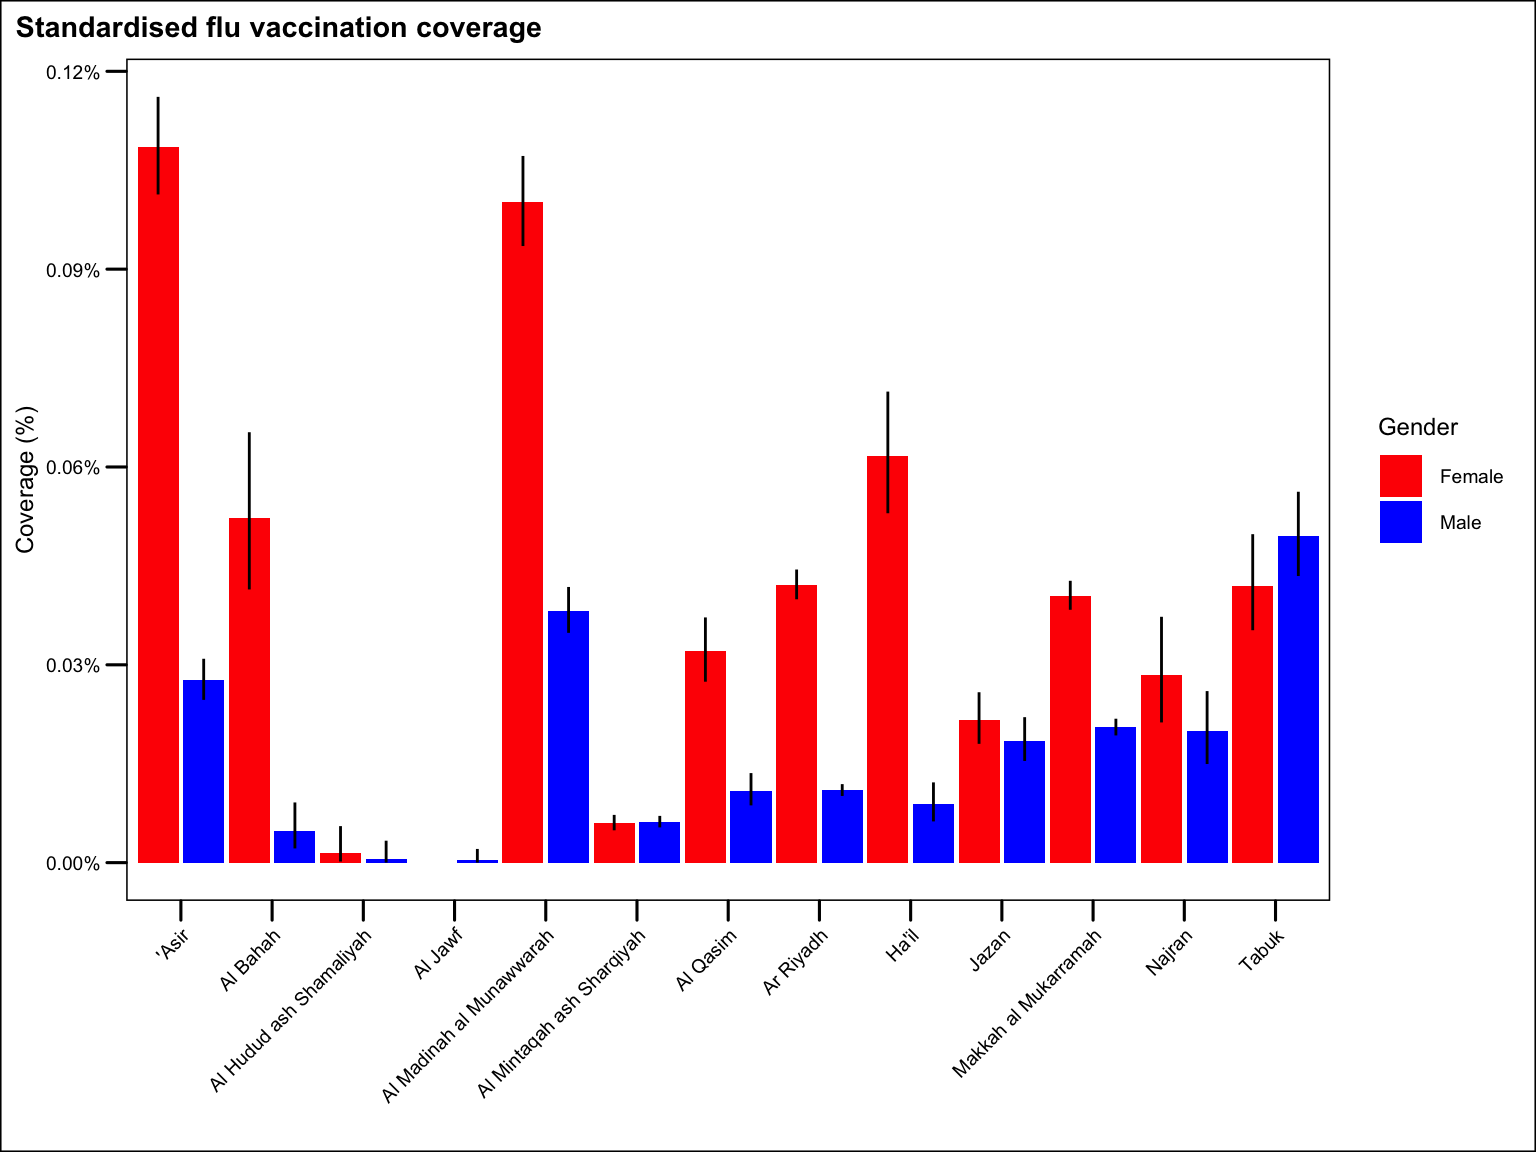
\includegraphics{flu_files/figure-pdf/calculate asr-1.pdf}

\bookmarksetup{startatroot}

\chapter{injury}\label{injury}

\subsection{Injury}\label{injury-1}

\bookmarksetup{startatroot}

\chapter{Summary}\label{summary}

In summary, this book has no content whatsoever.

\begin{Shaded}
\begin{Highlighting}[]
\DecValTok{1} \SpecialCharTok{+} \DecValTok{1}
\end{Highlighting}
\end{Shaded}

\begin{verbatim}
[1] 2
\end{verbatim}

\bookmarksetup{startatroot}

\chapter*{References}\label{references}
\addcontentsline{toc}{chapter}{References}

\markboth{References}{References}

\phantomsection\label{refs}
\begin{CSLReferences}{0}{1}
\end{CSLReferences}



\end{document}
